%\documentclass{beamer}
\documentclass[handout]{beamer}

%\setbeamerfont{author}{size=\tiny}
%\setbeamerfont{institute}{size=\tiny}

\setbeamertemplate{caption}{\raggedright\insertcaption\par}

\usepackage[latin1]{inputenc}
\usepackage{units}
\usepackage{soul}
\usepackage{comment}
\usepackage{minted}

%\usetheme{Warsaw}
\usetheme{CambridgeUS}

\title[ICTer 2023]{Forensic Insights from Electromagnetic Radiation}
%\title[Postgraduate Experience]{Standing on the Shoulders of Giants}
\subtitle{\footnotesize Workshop at ICTer Conference 2023}


\author[Asanka P. Sayakkara]{
	Dr.~Asanka P. Sayakkara \\ {\scriptsize{(asa@ucsc.cmb.ac.lk)}}
}

\institute[UCSC]{\scriptsize University of Colombo School of Computing\\Sri Lanka.}


%\author{Poshitha Dabare\inst{1}, Chathura Suduwella\inst{1}, Asanka Sayakkara\inst{1},\\Damitha Sandaruwan\inst{1}, Chamath Keppitiyagama\inst{1}, Kasun De Zoysa\inst{1},\\Kasun Hewage\inst{2} and Thiemo Voigt\inst{2,3}}
%\institute[shortinst]{\inst{1} University of Colombo School of Computing, Sri Lanka. \and %
%                      \inst{2} Uppsala University, Sweden. \and %
%                      \inst{3} SICS Swedish ICT, Sweden.}


\date{\tiny 10\textsuperscript{th} November, 2023}
%\subject{NBQSA, 2014}

\logo{%
  \makebox[0.95\paperwidth]{%
    %
\includegraphics[width=1cm,keepaspectratio]{figures/ucsc_image.pdf}%
    \hfill%
    
\includegraphics[width=1cm,keepaspectratio]{figures/ucsc_image.pdf}%
    %\hspace{3pt}
    %\includegraphics[width=0.9cm,keepaspectratio]{figures/uoc-logo.png}%
  }%
}

\begin{document}

%-------------------------------------------------------------------------------
\begin{frame}
\titlepage
\end{frame}
%-------------------------------------------------------------------------------

%-------------------------------------------------------------------------------
\begin{frame}{Asanka~P.~Sayakkara}  

	\begin{columns}
	
	\column{0.5\textwidth}
	
	\begin{itemize}
	\footnotesize
	\item BSc in Computer Science, University of Colombo School of Computing (UCSC), 2012.
	\vspace{10pt}
	\item PhD in Computer Science from University College Dublin, Ireland, 2020.
	\vspace{10pt}
	\item Forensic \& Security Research (ForSec) group of University College Dublin, Ireland,  2017--2020.
	\vspace{10pt}
	\item Senior lecturer at University of Colombo School of Computing (UCSC), Sri Lanka.
	\vspace{10pt}
	\item Coordinator of the MCS/MSc in CS degree programs.

	\end{itemize}


	\column{0.5\textwidth}

	\begin{figure}
		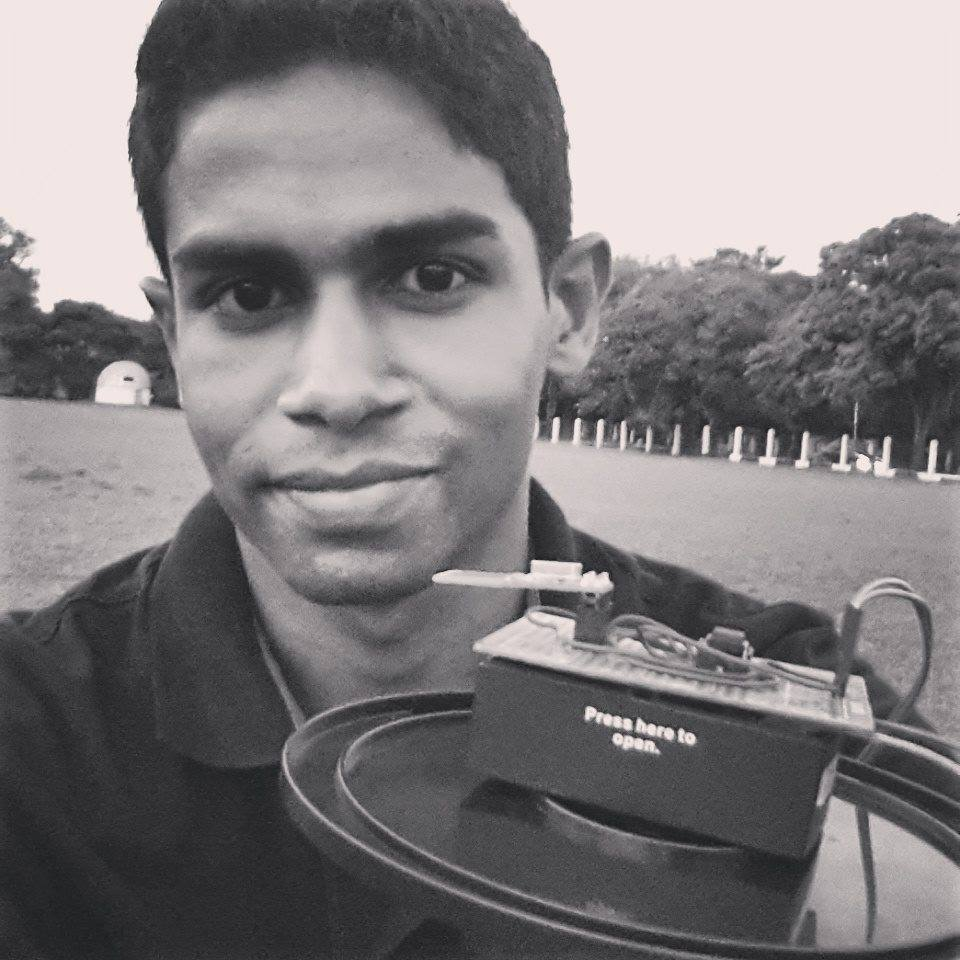
\includegraphics[width=80pt]{figures/me-with-mote.jpg}
	\end{figure}

	\begin{itemize}
	\footnotesize
	\item Introduction to Computing (FoS), Digital Forensics, Embedded Systems, and Operating Systems II.
	\vspace{10pt}
	\item Running \emph{Signal Insights} research lab.
	\vspace{10pt}
	\item {\scriptsize \url{https://ucsc.cmb.ac.lk/profile/asa} \\ \url{https://www.asayakkara.org}}
	\end{itemize}

	\end{columns}
\end{frame}
%-------------------------------------------------------------------------------


%-------------------------------------------------------------------------------
\begin{frame}{Signal Insights Research Lab}  

	\begin{figure}
		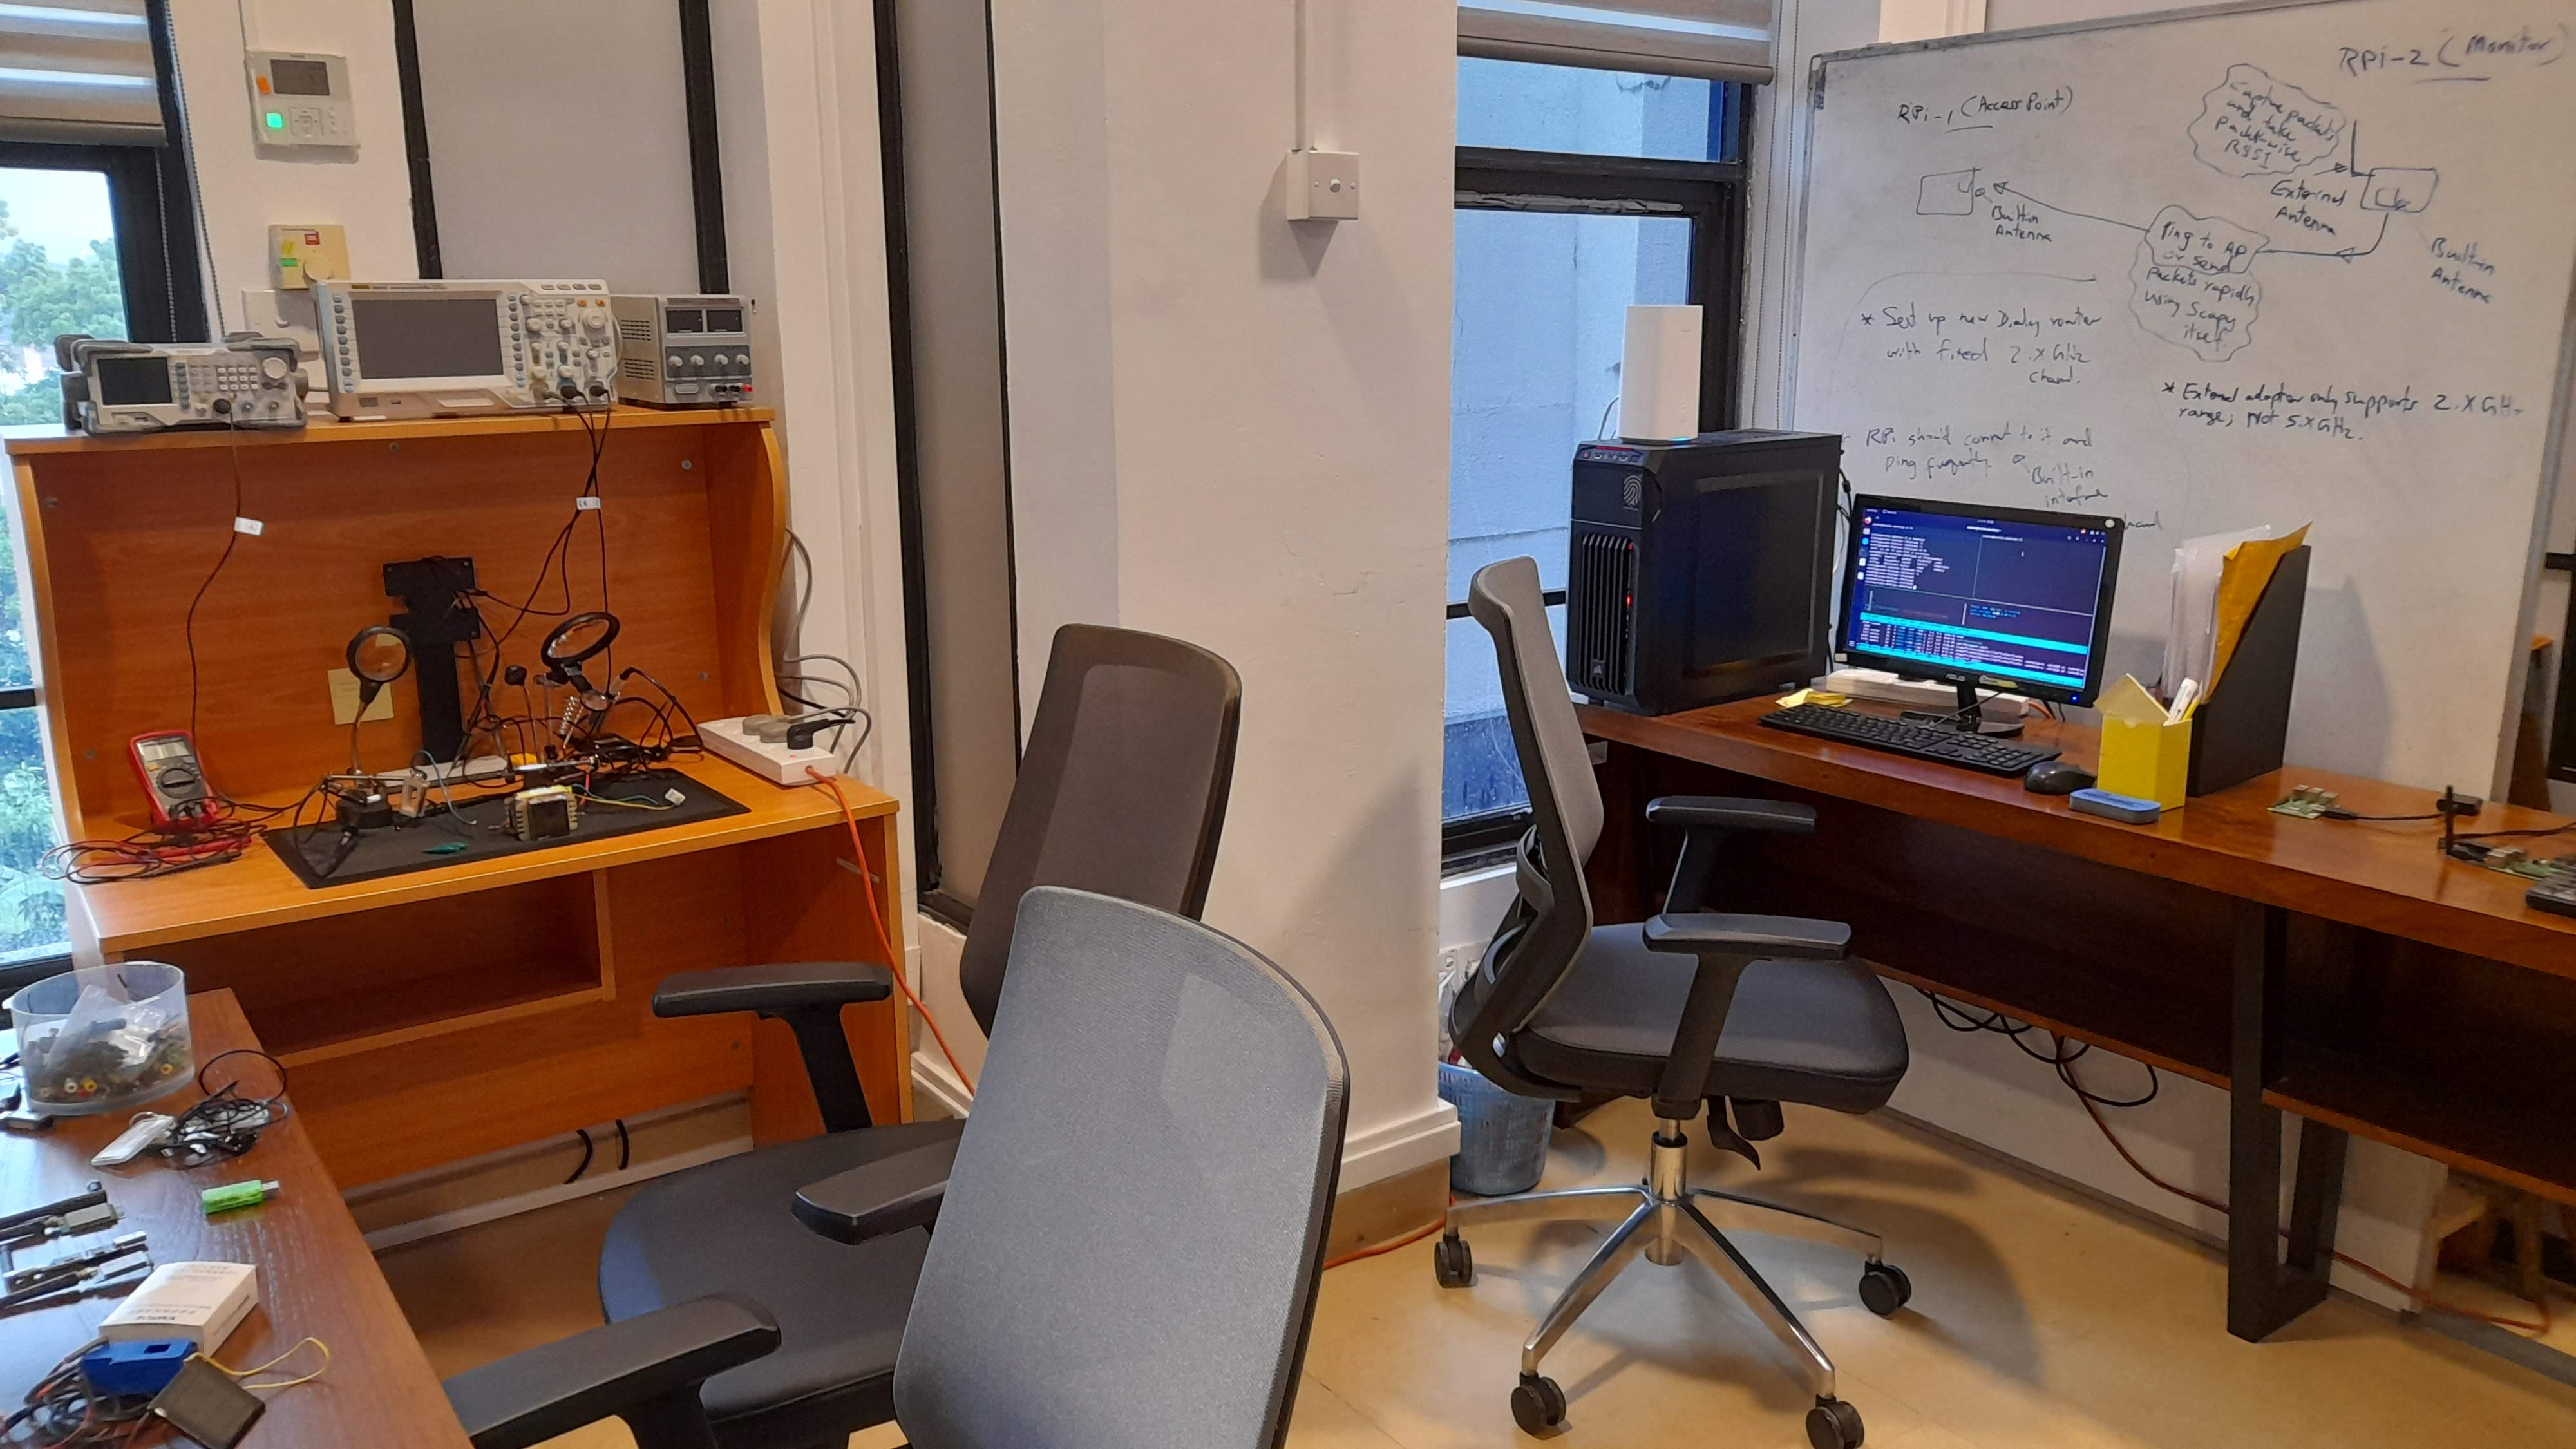
\includegraphics[width=180pt]{figures/signal-insights-lab-view.jpg}
	\end{figure}
	
	\begin{itemize}
		\footnotesize
		\item Potential of exploiting various signals originating from various sources.  
		\item Signal sources: artificial, as well as biological sources (bioacoustics).
		\item Electromagnetic side-channels and covert channels.
		\item Radio tomographic imaging.
		\item Passive acoustic monitoring (of elephants).
		\item {\scriptsize \url{https://www.asayakkara.org/signal-insights-lab.html}}
	\end{itemize}

\end{frame}
%-------------------------------------------------------------------------------


%-------------------------------------------------------------------------------
\begin{frame}{Workshop Agenda}  

\begin{columns}

\column{0.5\textwidth}

	\begin{itemize}
	\footnotesize
	\item \textbf{Part 1:}
		\begin{itemize}
		\footnotesize
		\item Hardware security.
		\item Digital forensics.
		\item Limitations of forensics.
		\item EM-SCA for forensics.
		\end{itemize}
		\vspace{10pt}
	\item \textbf{Part 2:}
		\begin{itemize}
		\footnotesize
    		\item SDR hardware.
    		\item SDR software.
		\end{itemize}
	\end{itemize}

\column{0.5\textwidth}

	\begin{itemize}
	\footnotesize
	\item \textbf{Part 3:}
		\begin{itemize}
		\footnotesize
    		\item EM trace data acquisition.
    		\item EM trace data processing.
		\end{itemize}
		\vspace{10pt}
	\item \textbf{Part 4:}
		\begin{itemize}
		\footnotesize
    		\item Exploring a large EM dataset.
    		\item Training ML models on EM data.
		\end{itemize}
	\end{itemize}

\end{columns}

\end{frame}
%-------------------------------------------------------------------------------


%-------------------------------------------------------------------------------
\begin{frame}{}  

	\begin{block}{Part 1}
	\end{block}

\end{frame}
%-------------------------------------------------------------------------------


%-------------------------------------------------------------------------------
\begin{frame}{Information Security}

\begin{itemize}
\footnotesize

\item Security is an essential element of modern computing systems.

%\vspace{10pt}

%\item Lack of security measures can result in the loss of money, fame, and trust.

%\vspace{10pt}

\end{itemize}

%\begin{columns}

%\column{0.3\textwidth}

\begin{figure}
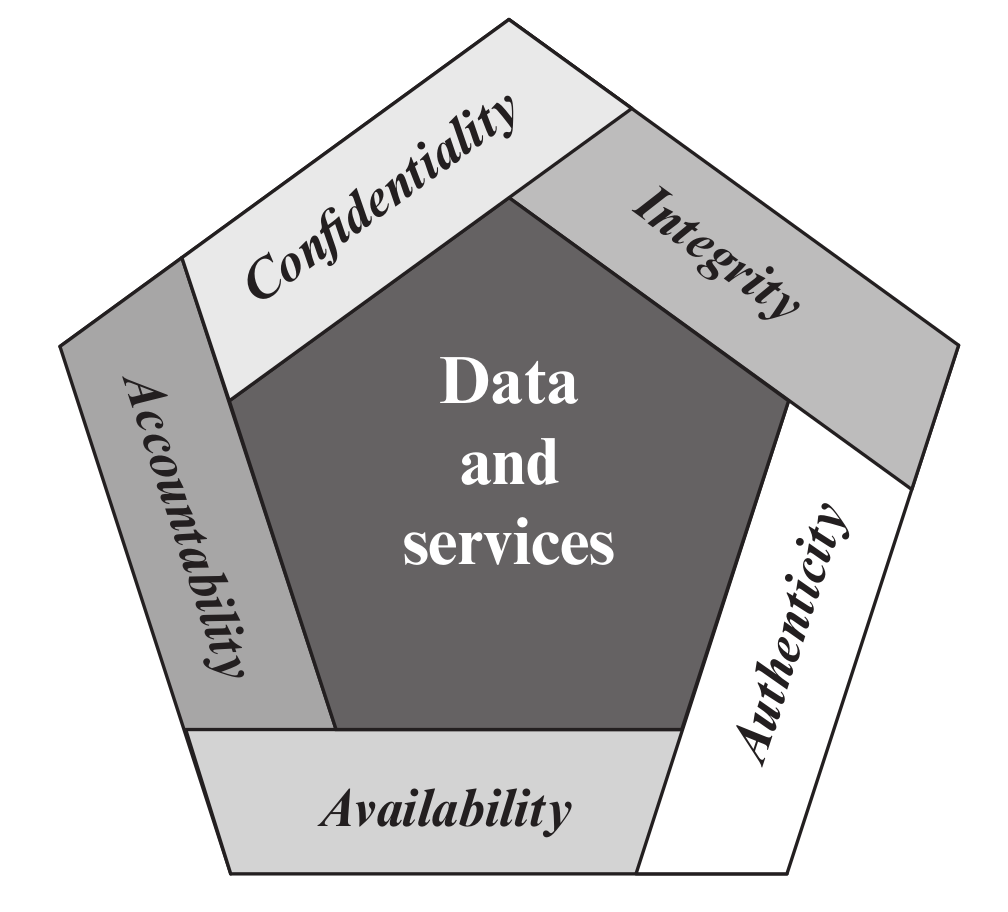
\includegraphics[width=160pt]{figures/security-requirements.png}
\end{figure}

%\column{0.7\textwidth}

%\begin{figure}
%\includegraphics[width=220pt]{figures/security-services-and-mechanisms.png}
%\end{figure}


%\end{columns}

\end{frame}
%-------------------------------------------------------------------------------


%-------------------------------------------------------------------------------
\begin{frame}{Hardware Security}

\begin{figure}
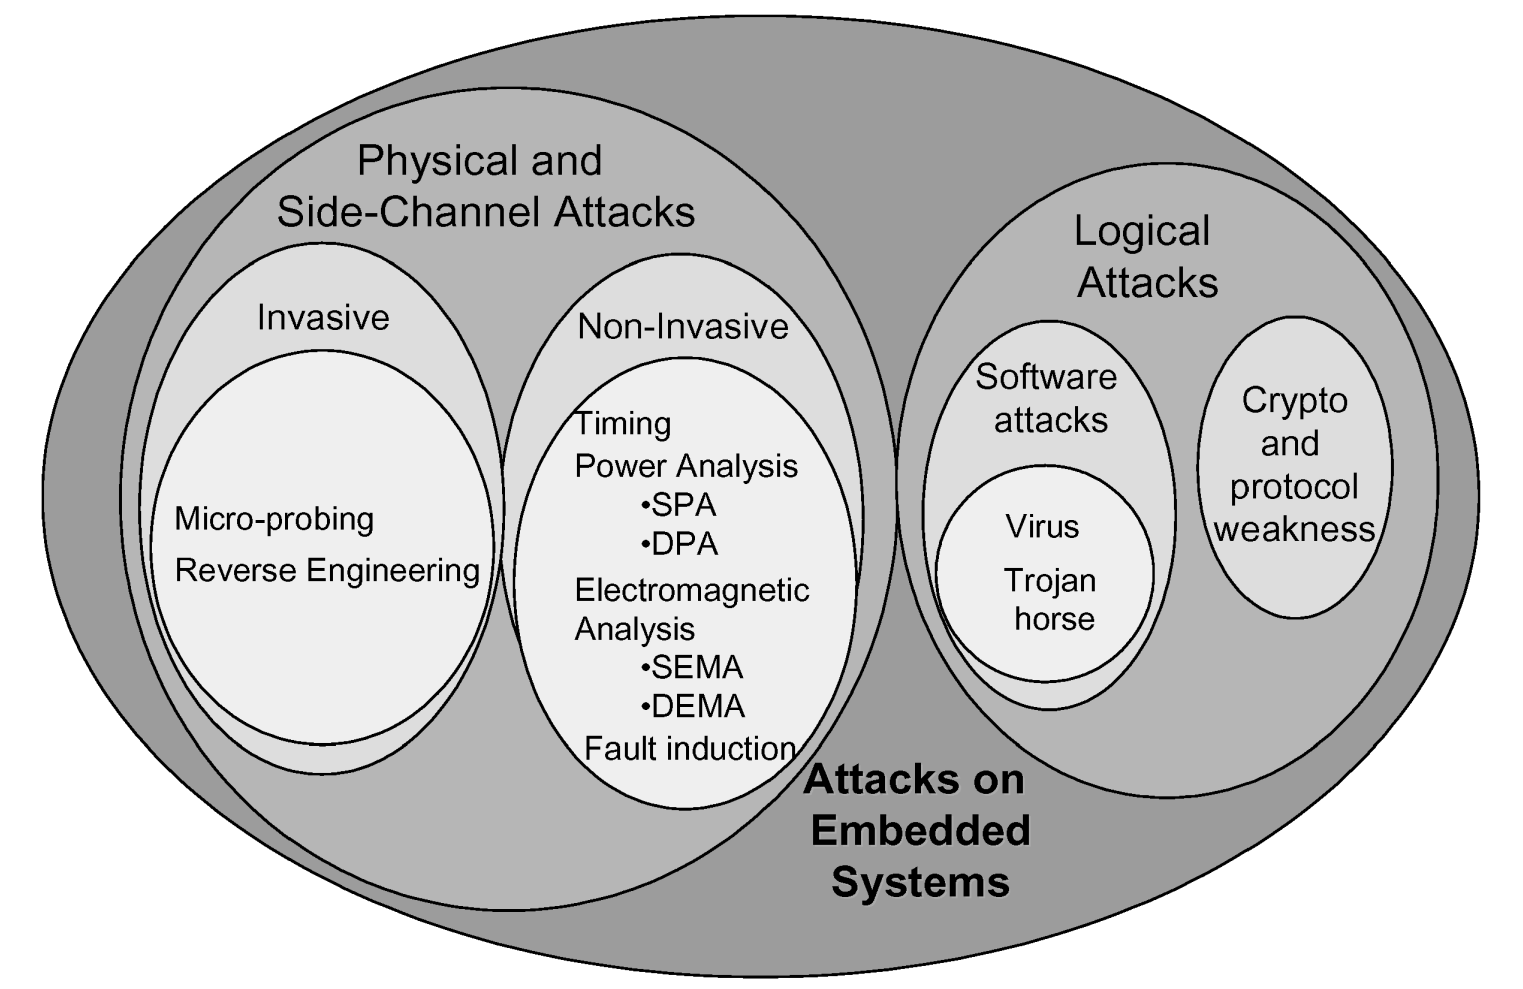
\includegraphics[width=260pt]{figures/attacks-on-embedded-systems.png}
\end{figure}

\end{frame}
%-------------------------------------------------------------------------------


%-------------------------------------------------------------------------------
\begin{frame}{Fault Injection Attacks}

\begin{itemize}
\footnotesize

\item Modern ICs are designed to work within specific operating ranges.

\vspace{10pt}

\item Faults arise whenever a deviation from the expected operating conditions occurs.

\vspace{10pt}

\item Of particular importance to security researchers are the errors produced by faults that can be used to compromise the security of computing devices.

\end{itemize}


\begin{columns}

\column{0.5\textwidth}

\begin{figure}
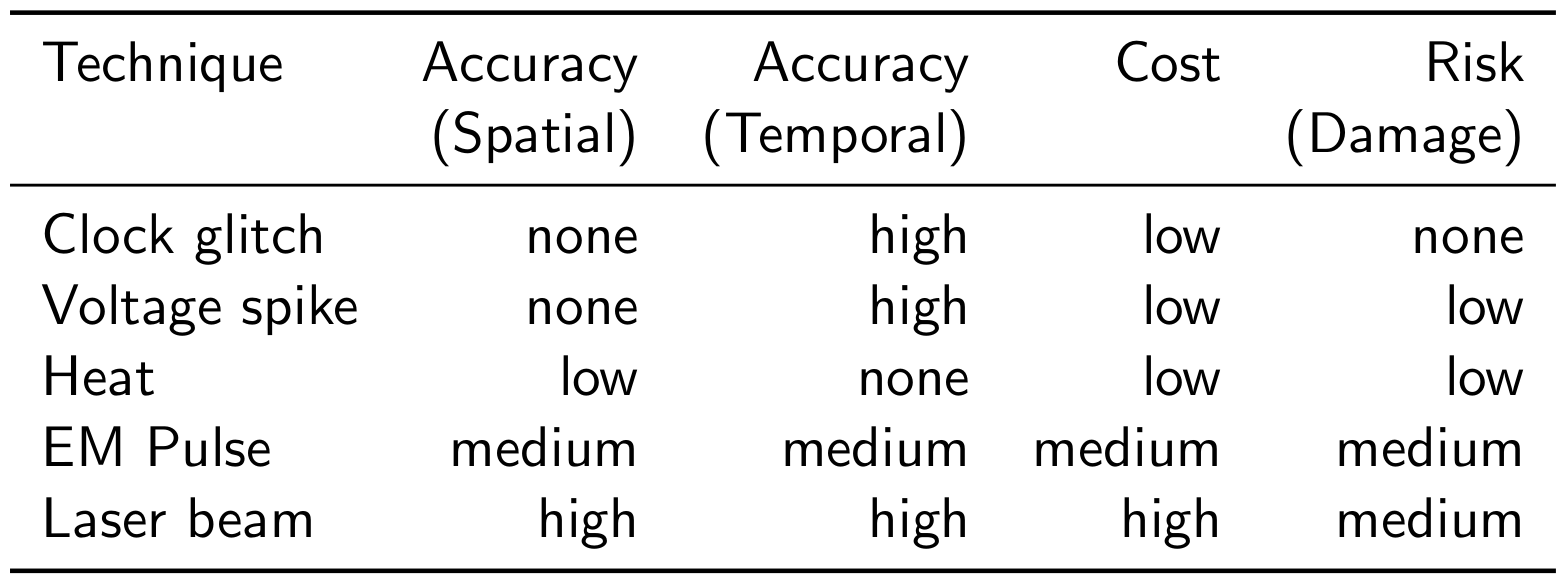
\includegraphics[width=170pt]{figures/fault-injection-techiques.png}
\end{figure}

\column{0.5\textwidth}

\begin{figure}
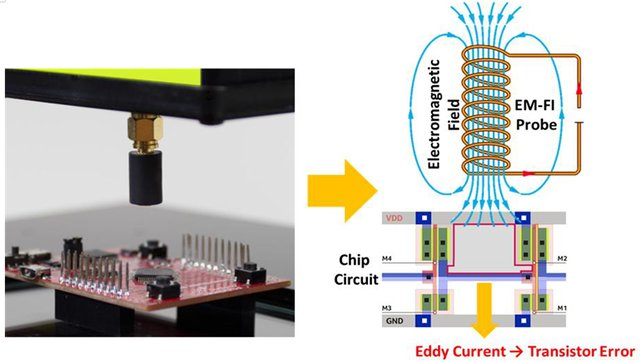
\includegraphics[width=170pt]{figures/Principle-of-electromagnetic-fault-injection.jpg}
\end{figure}

\end{columns}


\end{frame}
%-------------------------------------------------------------------------------

%-------------------------------------------------------------------------------
\begin{frame}{Side-Channel Analysis}

\begin{itemize}
\footnotesize

\item Data encryption algorithms are designed assuming that the intermediate data they are handling will not be available to third parties.

\vspace{10pt}

\item This assumption is not exactly correct for computers.

\vspace{10pt}

\item Information leakes through unintended channels from computers:
	\begin{itemize}
	\footnotesize
	\item Timing side-channel
	\item Acoustic side-channel
	\item Power side-channel
	\item Electromagnetic side-channel
	\end{itemize}

\vspace{10pt}

\item By exploiting such side-channels, attacks can be mounted at computing systems to extract confidential data.


\end{itemize}

\end{frame}
%-------------------------------------------------------------------------------

%-------------------------------------------------------------------------------
\begin{frame}{Simple Power Analysis -- SPA}

\begin{columns}

\column{0.6\textwidth}

\footnotesize
Identifying AES algorithm

\begin{figure}
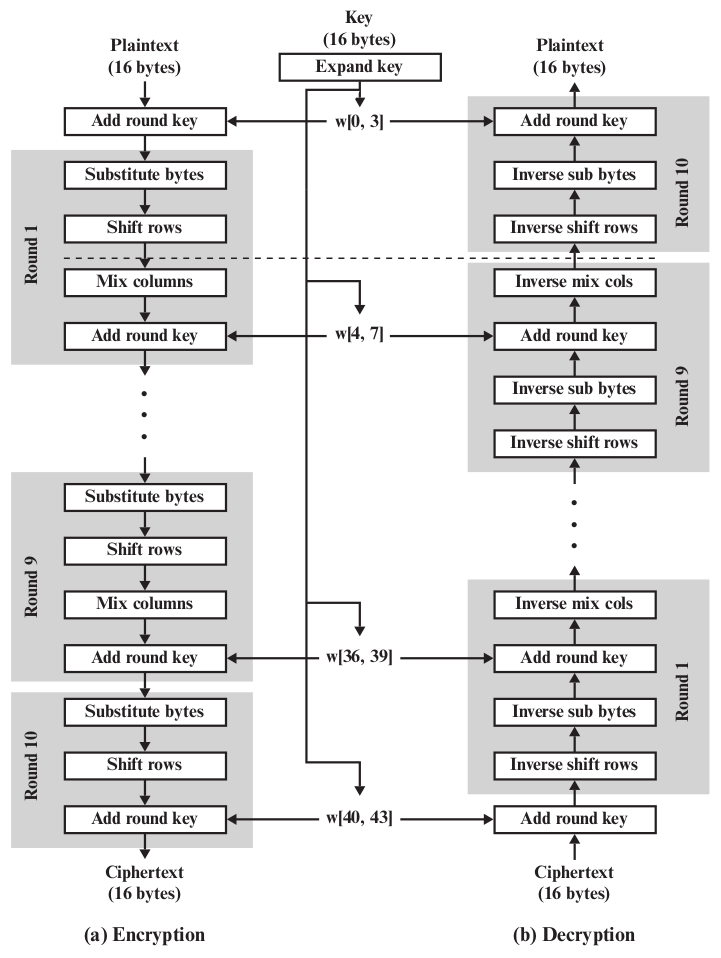
\includegraphics[width=140pt]{figures/aes-algorithm.png}
\end{figure}


\column{0.4\textwidth}

\begin{figure}
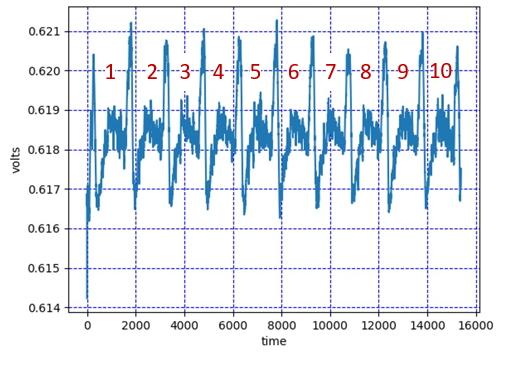
\includegraphics[width=110pt]{figures/aes-spa-trace.png}
\end{figure}

\begin{figure}
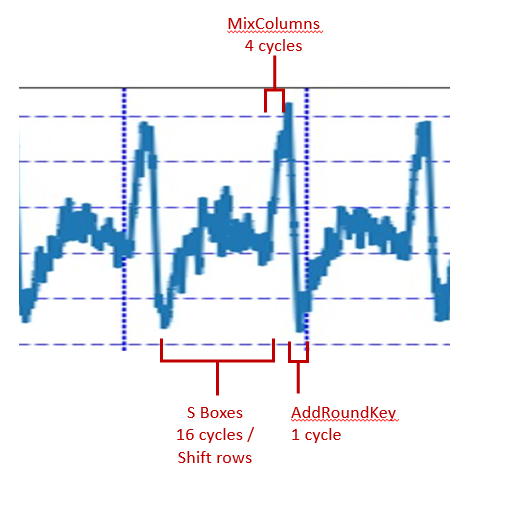
\includegraphics[width=110pt]{figures/aes-spa-trace-zoomed.png}
\end{figure}

\end{columns}

\end{frame}
%-------------------------------------------------------------------------------



%-------------------------------------------------------------------------------
\begin{frame}{Correlation Power Analysis -- CPA}

\begin{columns}

\column{0.5\textwidth}

\begin{itemize}
\footnotesize

\item Power consumption to retain a logic level 1 consumes more energy than logic level 0.

\vspace{10pt}

\item When a register holds some bit pattern, the \emph{hamming weight} gets reflected in the energy consumption (and EM radiation too).

\vspace{10pt}

\item The Correlation Power Analysis (CPA) exploits this phenomena to identify the unknown bit pattern of the secret key.

\end{itemize}

\column{0.5\textwidth}

\begin{figure}
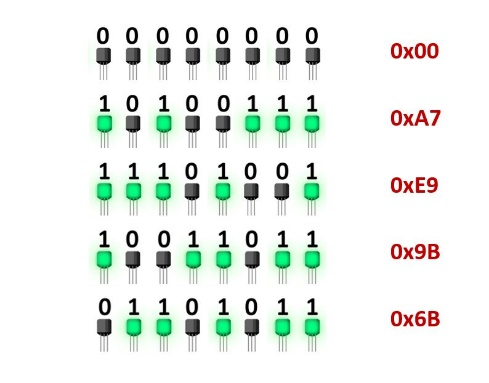
\includegraphics[width=150pt]{figures/hamming-weight-illustration.png}
\end{figure}

\end{columns}

\end{frame}
%-------------------------------------------------------------------------------


%-------------------------------------------------------------------------------
\begin{frame}{Correlation Power Analysis (cont.)}

\begin{columns}

\column{0.5\textwidth}

\begin{figure}
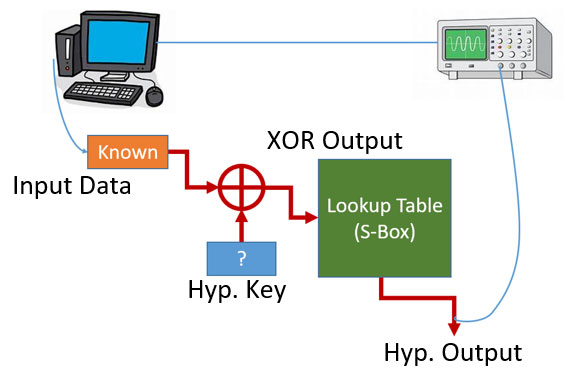
\includegraphics[width=150pt]{figures/cpa-measurement-setup.png}
\end{figure}

\column{0.5\textwidth}


\begin{figure}
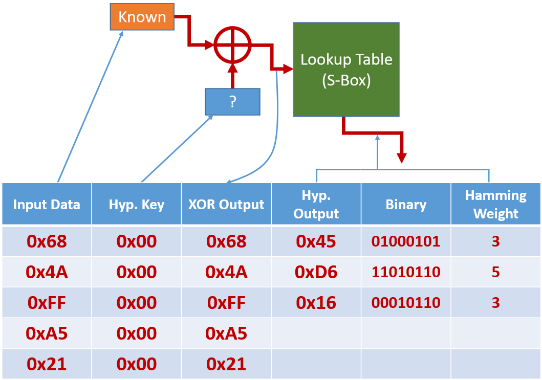
\includegraphics[width=150pt]{figures/cpa-measurement-data.png}
\end{figure}

\end{columns}

\begin{figure}
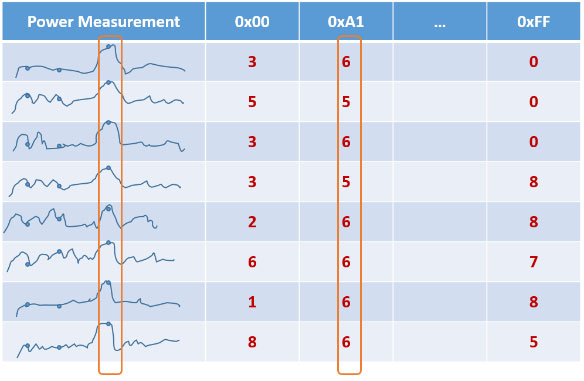
\includegraphics[width=150pt]{figures/cpa-measurement-correlation.png}
\end{figure}


\end{frame}
%-------------------------------------------------------------------------------


%-------------------------------------------------------------------------------
\begin{frame}{Correlation Power Analysis (cont.)}

\footnotesize
Take a look at the simulated CPA attack in the Jupyter Notebook.

\end{frame}
%-------------------------------------------------------------------------------

%-------------------------------------------------------------------------------
\begin{frame}{Electromagnetic Side-Channel Analysis}  

	\begin{itemize}
	\footnotesize
	\item Time-varying electrical currents are generating electromagnetic (EM) radiation.
		\vspace{10pt}
	\item Our electronic equipment are a source of strong EM radiation.
		\vspace{10pt}
	\item The EM radiation of computers (specifically, the processors) is shown to be correlating with the software running on them, i.e., the exact instructions and their execution pattern.
		\vspace{10pt}
	\item EM Side-Channel Analysis (EM-SCA) is the exploitation of these radiation to eavesdrop on computers:
		\vspace{5pt}
		\begin{itemize}
		\footnotesize
		\item Software behaviour dection.
		\vspace{10pt}
		\item Malicious firmware modification detection.
		\vspace{10pt}
		\item Cryptographic key retrieval.
		\end{itemize}
	\end{itemize}

\end{frame}
%-------------------------------------------------------------------------------


%-------------------------------------------------------------------------------
\begin{frame}{Electromagnetic Side-Channel Analysis (cont.)}  

\footnotesize
A Few Demonstrations
\vspace{10pt}

\begin{itemize}
	\footnotesize
	\item Radiation from the laptop screen/graphic card:\\ \url{https://www.youtube.com/watch?v=YtolwTPDBwk}
	\vspace{10pt}
	\item Remote servelliance of video displays:\\ \url{http://www.youtube.com/watch?v=8OlkywZBJGU}
	\vspace{10pt}
	\item Data exfiltration through EM covert channel on an Ethernet cable:\\ \url{https://www.youtube.com/watch?v=ciM4M5h3q0w}
	\vspace{10pt}
	\item A clock glitch attack on Arduino Uno:\\ \url{https://www.youtube.com/watch?v=Me9Kf2Ga0vs}
	\vspace{10pt}
	\item Intercepting smart card communication using HackRF One:\\ \url{https://www.youtube.com/watch?v=HiUu3\_3kQYY}
\end{itemize}

\end{frame}
%-------------------------------------------------------------------------------


%-------------------------------------------------------------------------------
\begin{frame}{Old Incidents and Crimes}

\begin{figure}
   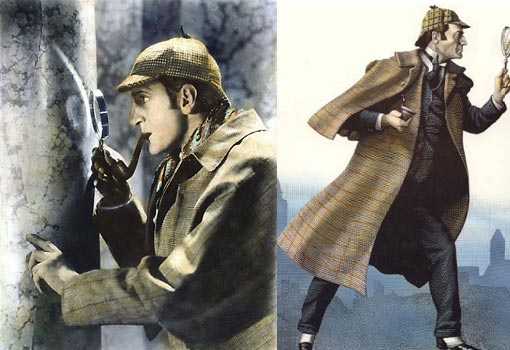
\includegraphics[width=3in]{figures/old-incidents.jpg}
\end{figure}

\pause
\footnotesize
Fingerprints, bloodstains, hand-written notes, eye witness, etc.

\end{frame}
%-------------------------------------------------------------------------------



%-------------------------------------------------------------------------------
\begin{frame}{Modern Incidents and Crimes}

\begin{figure}
   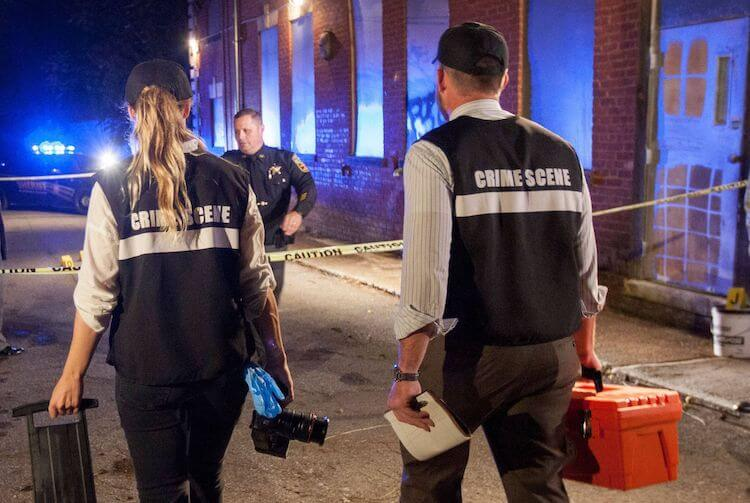
\includegraphics[width=3in]{figures/modern-incidents.jpeg}
\end{figure}

\pause
\footnotesize
DNA analysis, biometrics, CCTV footage, facial recognition, etc.

\end{frame}
%-------------------------------------------------------------------------------

%-------------------------------------------------------------------------------
\begin{frame}{Digital Forensics}

\begin{figure}
   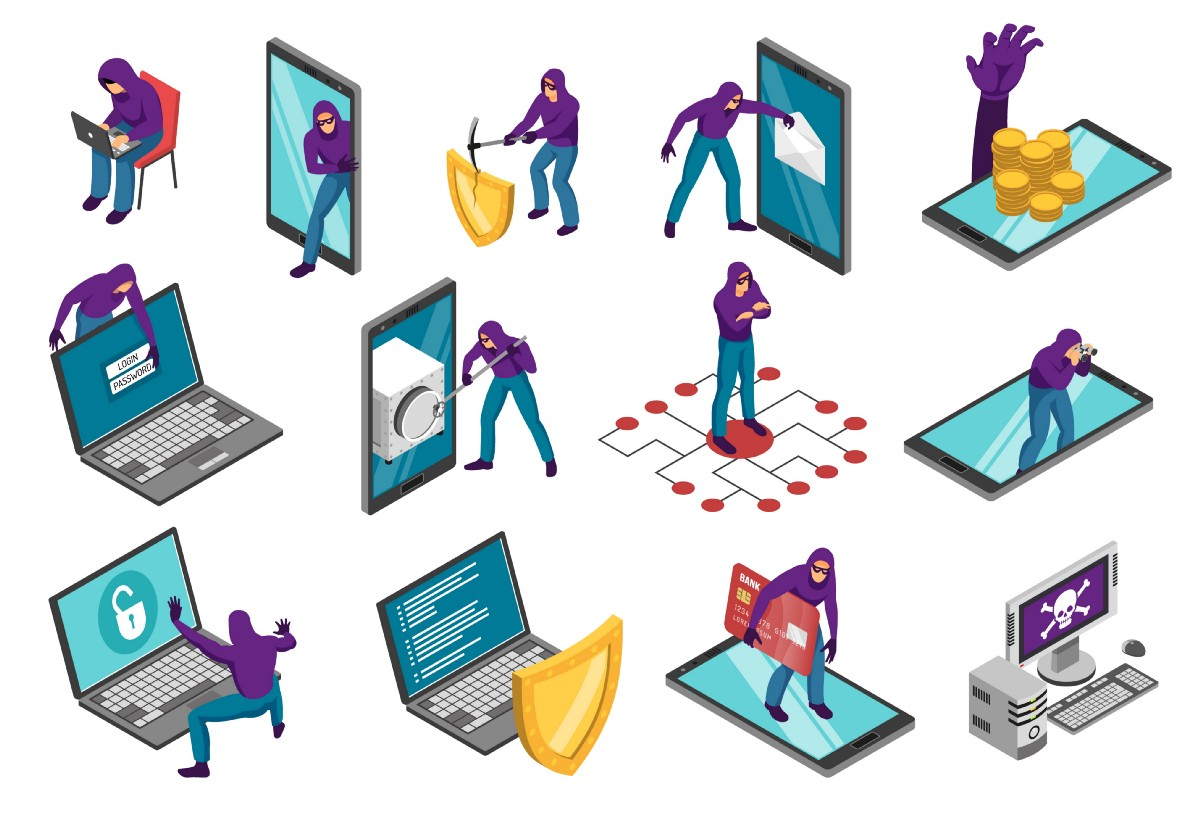
\includegraphics[width=3in]{figures/digital-forensics.jpeg}
\end{figure}


\end{frame}
%-------------------------------------------------------------------------------



%-------------------------------------------------------------------------------
\begin{frame}{Digital Evidence}

\begin{figure}
   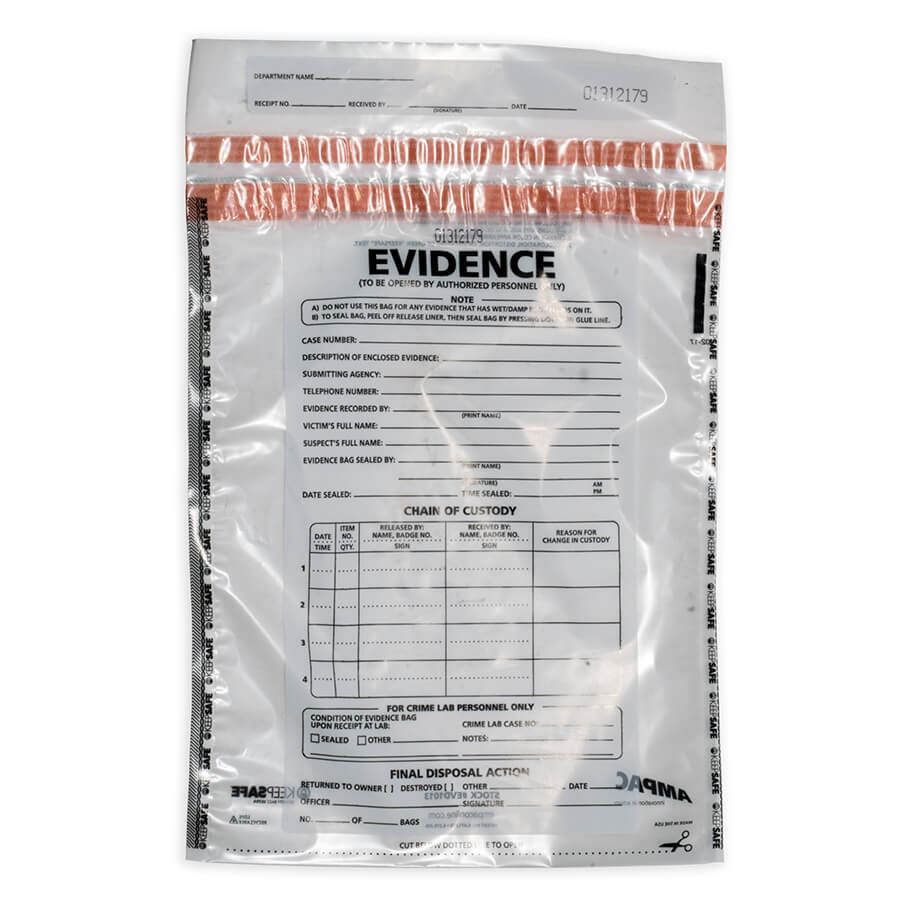
\includegraphics[width=2in]{figures/digital-evidence.jpg}
\end{figure}

\pause
\footnotesize
Any data stored or transmitted using a computer that support or refute a theory of how an offense occurred or that address critical elements of the offense.


\end{frame}
%-------------------------------------------------------------------------------


%-------------------------------------------------------------------------------
\begin{frame}{Digital Evidence Sources}

\begin{itemize}
\footnotesize
\item Open computer systems (laptops, desktops, smartphones, and their storage devices).
\vspace{10pt}
\item Embedded computer systems (smart wearables, printers, access control systems, etc.).
\vspace{10pt}
\item Communication systems (wired and wireless network data).
\end{itemize}

\end{frame}
%-------------------------------------------------------------------------------



%-------------------------------------------------------------------------------
\begin{frame}{Chain of Custody}

\begin{figure}
   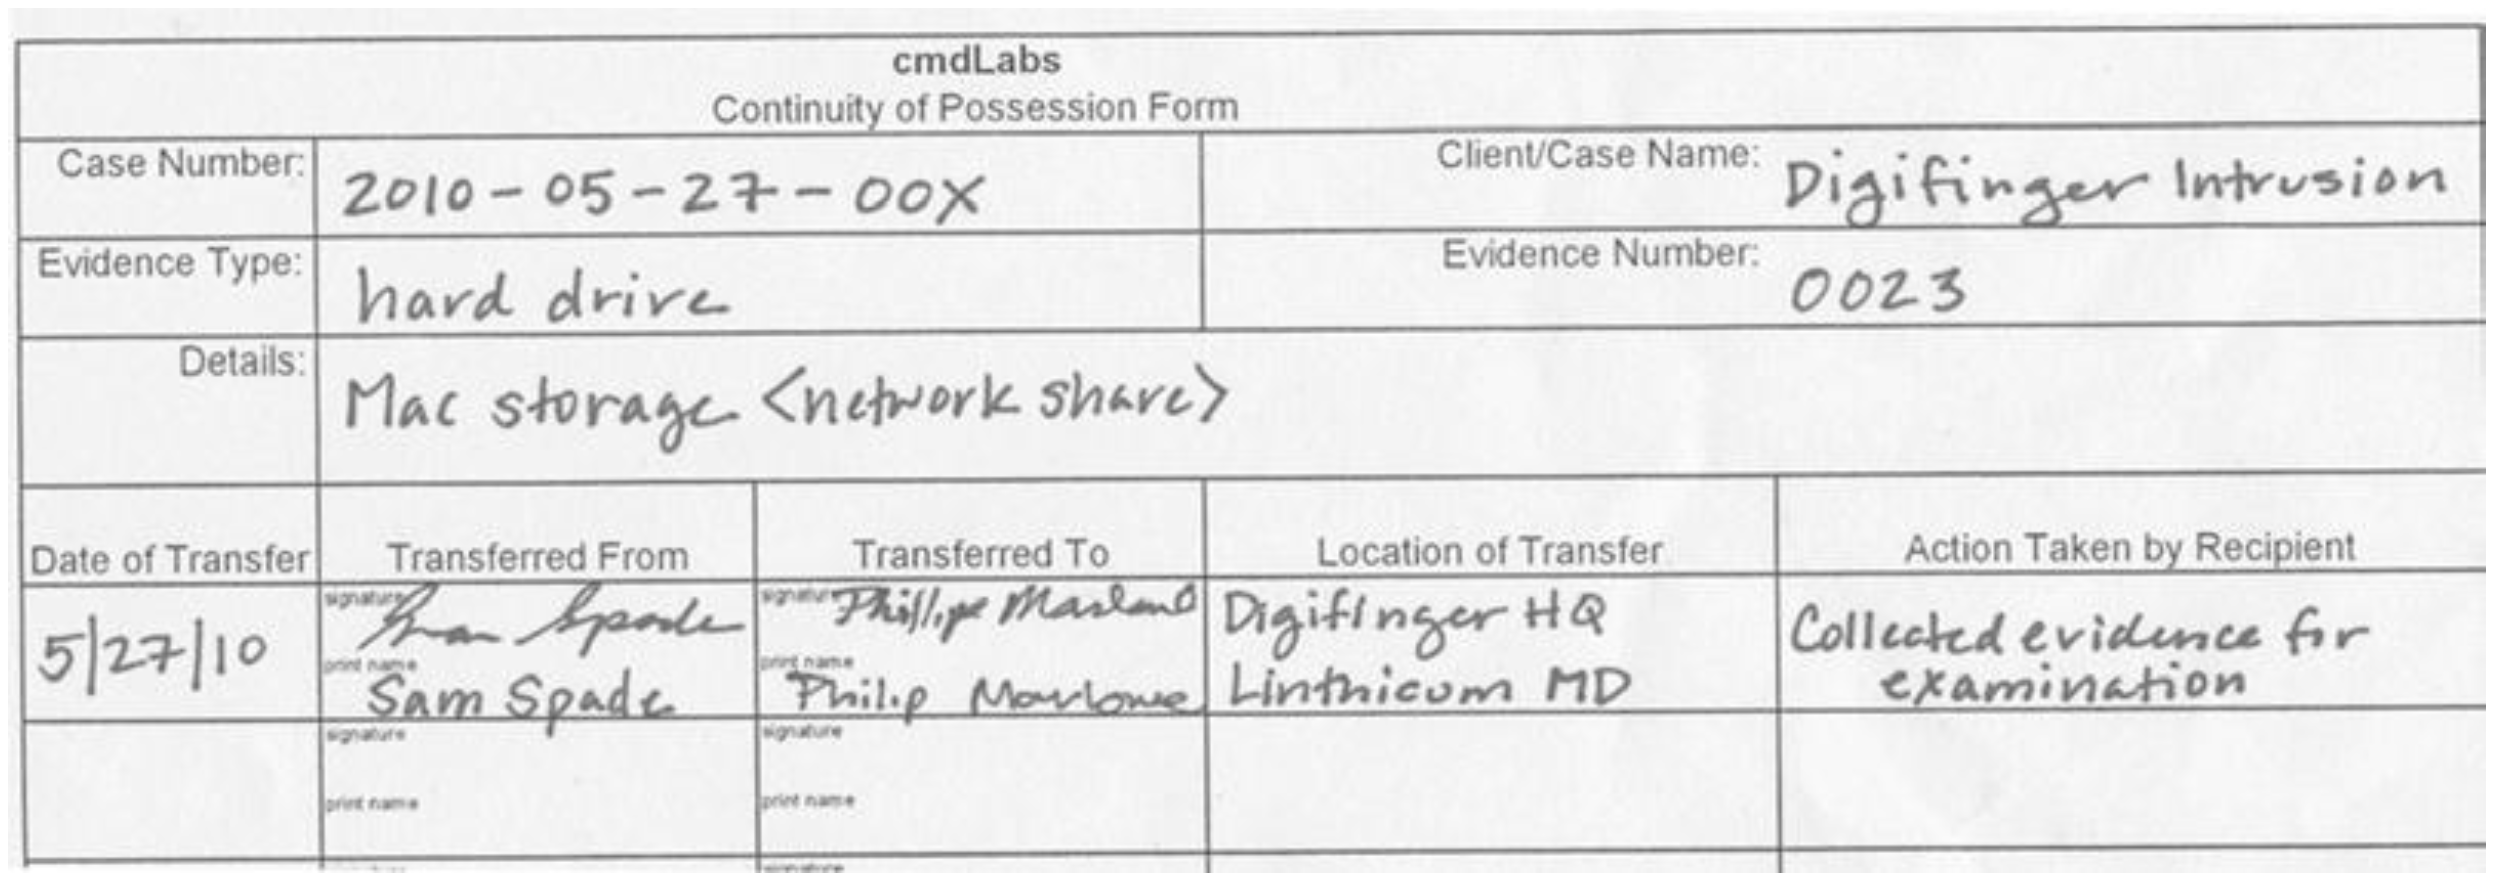
\includegraphics[width=4in]{figures/chain-of-custody-form.png}
\end{figure}

\end{frame}
%-------------------------------------------------------------------------------


%-------------------------------------------------------------------------------
\begin{frame}{Digital Forensics Process}

\begin{figure}
   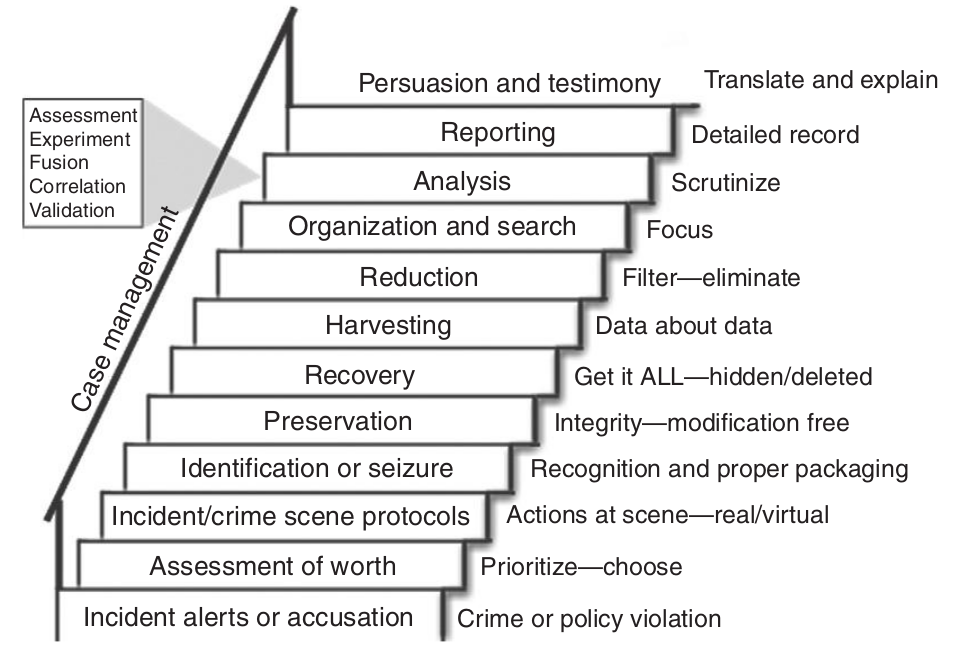
\includegraphics[width=3.5in]{figures/digital-forensics-process.png}
\end{figure}

\end{frame}
%-------------------------------------------------------------------------------


%-------------------------------------------------------------------------------
\begin{frame}{`Science' in Digital Forensics}

\begin{columns}

\column{0.5\textwidth}

\begin{itemize}
\footnotesize
\item Forensics is a scientific discipline --- so as digital forensics.
\vspace{10pt}
\item A scietific discipline should follow the \textbf{scientific method}.
\vspace{10pt}
\item Repeatability and Reproducibility
\vspace{10pt}
\item Elimination of hypotheses.
\end{itemize}

\column{0.5\textwidth}

\begin{figure}
   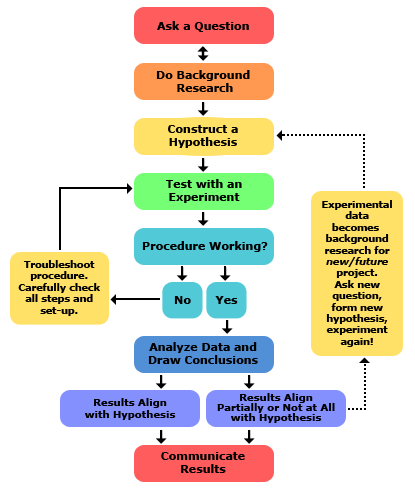
\includegraphics[width=160pt]{figures/scientific-method.png}
\end{figure}

\end{columns}

\end{frame}
%-------------------------------------------------------------------------------


%-------------------------------------------------------------------------------
\begin{frame}{ACPO Guidelines}

\begin{itemize}
\footnotesize

\item If a digital crime scene is not handled properly, the entire operations afterwards will be futile.
\vspace{10pt}

\item Various standards exists on how to handle a digital crime scene.
\vspace{10pt}

\item The \emph{Association for Chief Police Officers} (ACPO), has published a guide of good practices, which is highly recognised.
\vspace{10pt}

\item These are not strict rules, but helpful guidelines --- under certain conditions we may have to deviate from them.

\end{itemize}

\end{frame}
%-------------------------------------------------------------------------------


%-------------------------------------------------------------------------------
\begin{frame}{ACPO Guidelines}

\begin{itemize}
\footnotesize

\item \textbf{Principle 1:} No action taken by law enforcement agencies or their agents should change data held on a computer or storage media which may subsequently be relied upon in court.
\vspace{10pt}

\item \textbf{Principle 2:} In circumstances where a person finds it necessary to access original data held on a computer or on storage media, that person must be competent to do so and be able to give evidence explaining the relevance and the implications of their actions.
\vspace{10pt}

\item \textbf{Principle 3:} An audit trail or other record of all processes applied to computer-based electronic evidence should be created and preserved. An independent third party should be able to examine those processes and achieve the same result.
\vspace{10pt}

\item \textbf{Principle 4:} The person in charge of the investigation (the case officer) has overall responsibility for ensuring that the law and these principles are adhered to.

\end{itemize}

\end{frame}
%-------------------------------------------------------------------------------



%-------------------------------------------------------------------------------
\begin{frame}{Challenge of IoT \& Smart Device Forensics}  

	\begin{figure}
		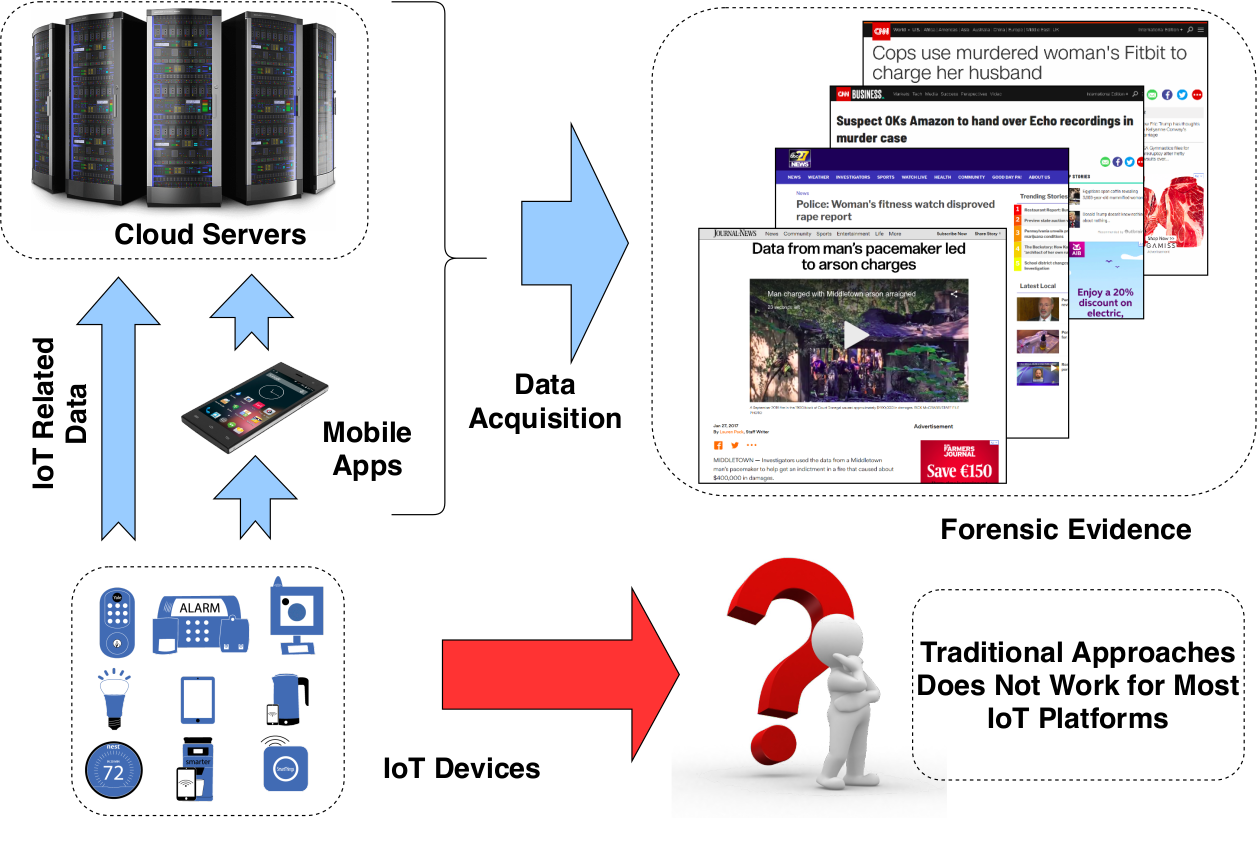
\includegraphics[width=250pt]{figures/IoT-forensic-challenge-small.png}
	\end{figure}

\end{frame}
%-------------------------------------------------------------------------------


%-------------------------------------------------------------------------------
\begin{frame}{Challenge of IoT \& Smart Device Forensics (cont.)}  

\begin{itemize}
\footnotesize
\item New devices are emerging in the market too frequently.
\vspace{10pt}
\item The internal components, storage, and interfaces of the devices varies drastically.
\vspace{10pt}
\item Analysing devices at too close to the hardware level --- such as chip-off forensics --- is susceptibe to irreversible mistakes that can destroy a device entirely.
\vspace{10pt}
\item It would be ideal if we can inspect a device from a safe distance.
\end{itemize}

\end{frame}
%-------------------------------------------------------------------------------



%-------------------------------------------------------------------------------
\begin{frame}{Evidence vs Insights}  

\begin{columns}

	\column{0.4\textwidth}

	\begin{figure}
		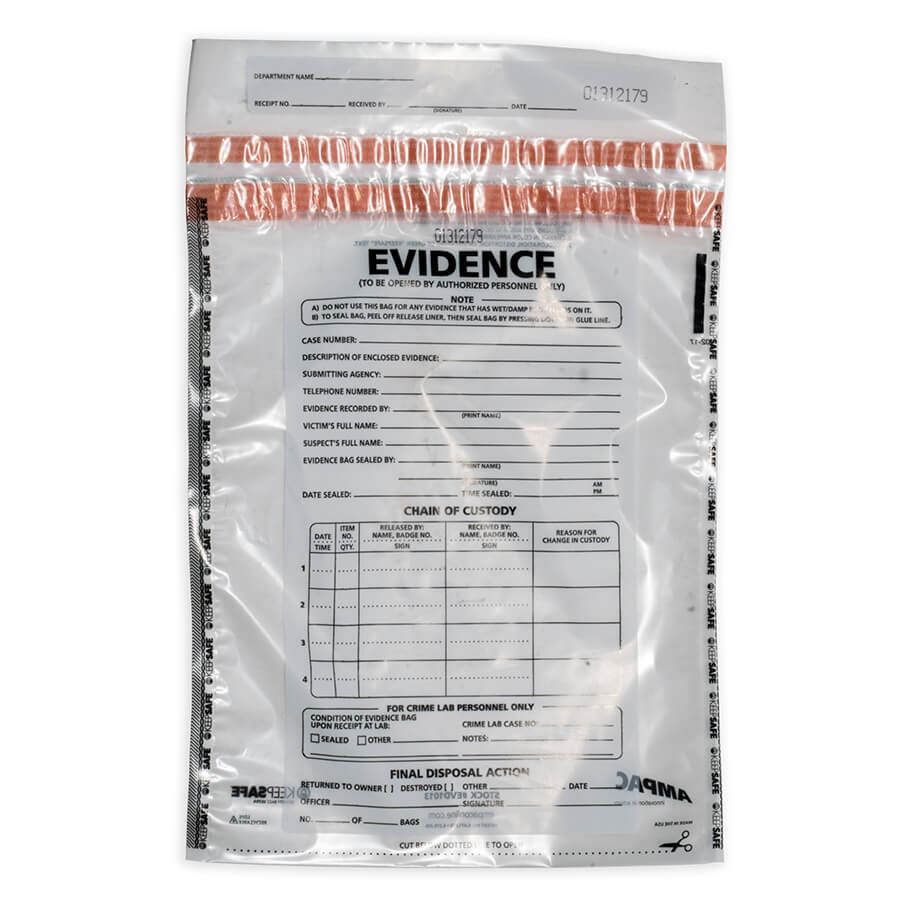
\includegraphics[width=150pt]{figures/digital-evidence.jpg}
	\end{figure}

	\column{0.6\textwidth}

	\begin{itemize}
	\footnotesize
	\item Digital \textbf{evidence} are information that may be presented to a court of law.
		\vspace{10pt}
	\item They need to be concrete enough to be relied upon at the courts.
		\vspace{10pt}
	\item The field of digital forensics is aimed at providing this reliability as much as possibile.
		\vspace{10pt}
	\item In some situations, where evidence are not available, some \textbf{insights} can a lifeline for an investigator. 
		\vspace{10pt}
	\item Insights are --- most likely --- not reproducible, but they can provide useful hints and directions to go and locate reliable evidence through other means. 
	\end{itemize}

\end{columns}

\end{frame}
%-------------------------------------------------------------------------------


%-------------------------------------------------------------------------------
\begin{frame}{Forensic Insights from IoT and Smart Devices}  

	\begin{itemize}
	\footnotesize
	\item Is this device running the official firmware from the manufacturer?
		\vspace{10pt}
	\item Has a malware been injected to the memory of this device?
		\vspace{10pt}
	\item Is this device doing something it is not supposed to be doing right now; such as wiping the storage or encrypting it, instead of shutting down?
	\end{itemize}

\end{frame}
%-------------------------------------------------------------------------------


%-------------------------------------------------------------------------------
\begin{frame}{Forensic Insights through EM-SCA}  

	\begin{figure}
		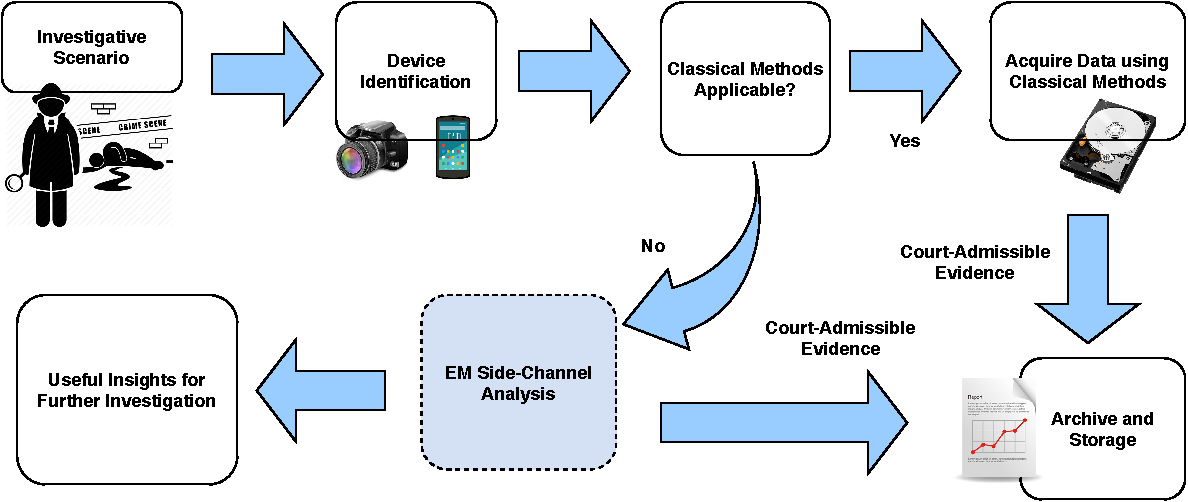
\includegraphics[width=280pt]{figures/applying-em-sca-to-forensic-process.pdf}
	\end{figure}

\end{frame}
%-------------------------------------------------------------------------------



%-------------------------------------------------------------------------------
\begin{frame}{}  

	\begin{block}{Part 2}
	\end{block}

\end{frame}
%-------------------------------------------------------------------------------


%-------------------------------------------------------------------------------
\begin{frame}{Radio/Wireless Devices}  

\begin{itemize}
	\footnotesize
	\item Built using hardware components that deal with analog signals.
	\vspace{10pt}
	\item Digitisation (if any) occurs in a very late stage.
	\vspace{10pt}
	\item Application-specific hardware configurations.
\end{itemize}

	\begin{figure}
		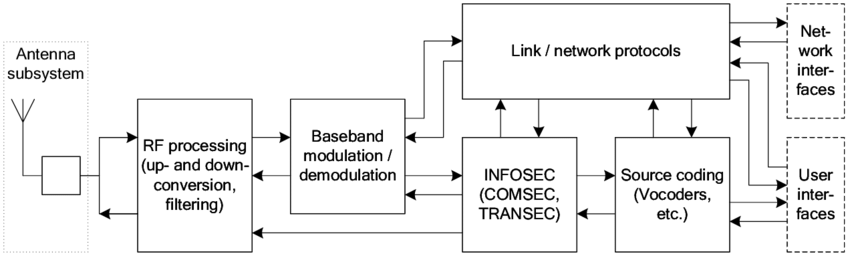
\includegraphics[width=290pt]{figures/Radio-architecture-functional-overview.png}
	\end{figure}

\end{frame}
%-------------------------------------------------------------------------------


%-------------------------------------------------------------------------------
\begin{frame}{Software Defined Radios}  

\begin{itemize}
	\footnotesize
	\item Moving most of radio functions from analog domain into the digital domain.
	\vspace{10pt}
	\item Requires a generic hardware radio interface including a fast analog-to-digital converter (ADC).
	\vspace{10pt}
	\item Involves a local oscillator (LO) with a mixer --- not illustrated in the figure.
	\vspace{10pt}
	\item Need sophisticated and optimised software implementations for digital signal processing (DSP).
\end{itemize}

	\begin{figure}
		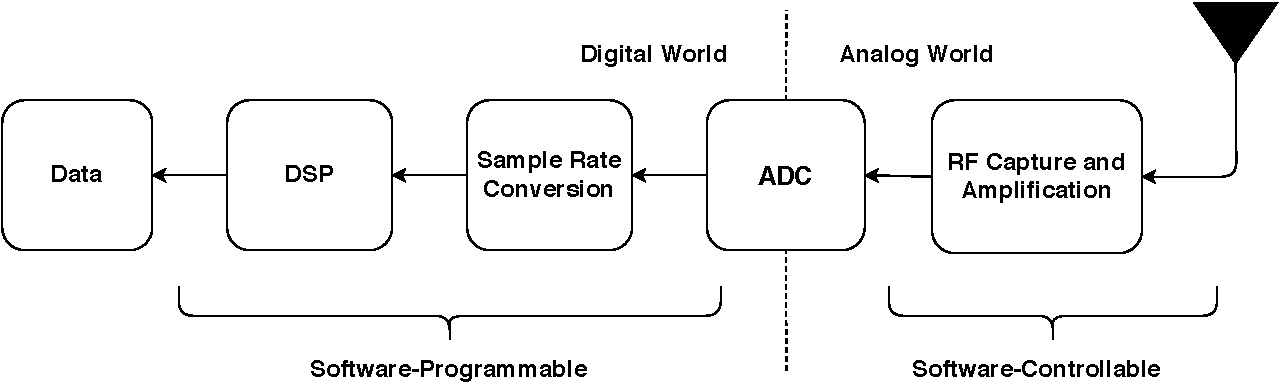
\includegraphics[width=290pt]{figures/sdr-architecture.pdf}
	\end{figure}

\end{frame}
%-------------------------------------------------------------------------------


%-------------------------------------------------------------------------------
\begin{frame}{Software Defined Radios (cont.)}  

	\footnotesize
	Converting analog signals to digital signals require \textbf{sampling} and \textbf{quantisation}. 

	\begin{figure}
		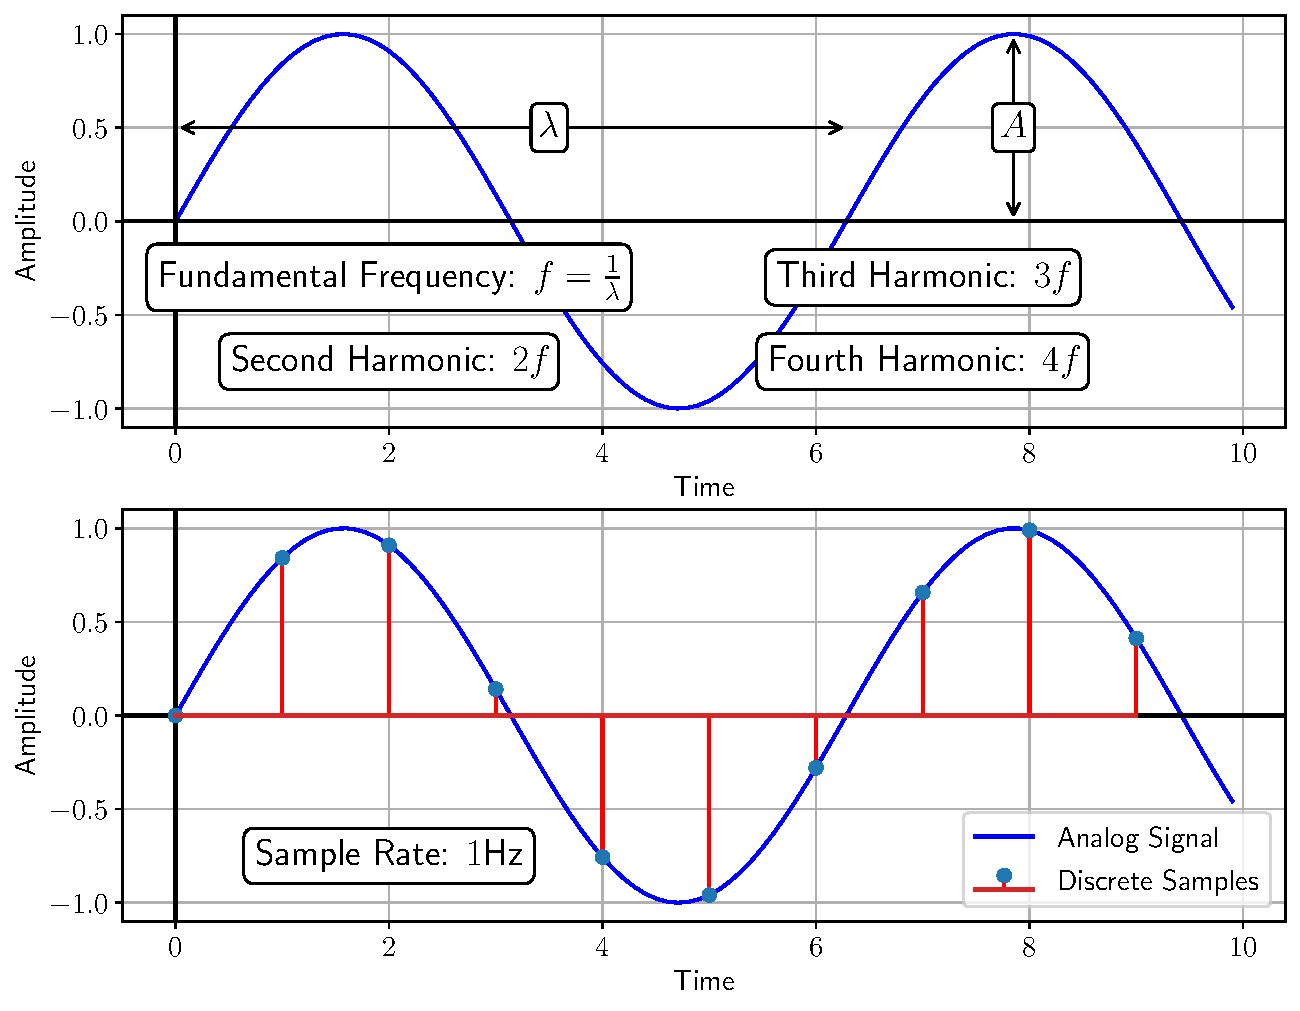
\includegraphics[width=210pt]{figures/signal-properties.pdf}
	\end{figure}

	\footnotesize
	\textbf{Real-valued sampling} faces the Nyquist limit: difficult to capture high frequencies.

\end{frame}
%-------------------------------------------------------------------------------


%-------------------------------------------------------------------------------
\begin{frame}{Software Defined Radios (cont.)}  

	\begin{itemize}
	\footnotesize
	\item SDRs are using complex \textbf{In-phase/Quadrature (I/Q)} sampling.
		\vspace{5pt}
	\item Each sample taken at a given time instance consists of two values; hence, each sample is a complex number.
		\vspace{5pt}
	\item A EM signal captured by an SDR is basically an array of complex numbers.
		\vspace{5pt}
	\item Sampling rate is equal to the bandwidth of the captured data.
	\end{itemize}

	\begin{figure}
		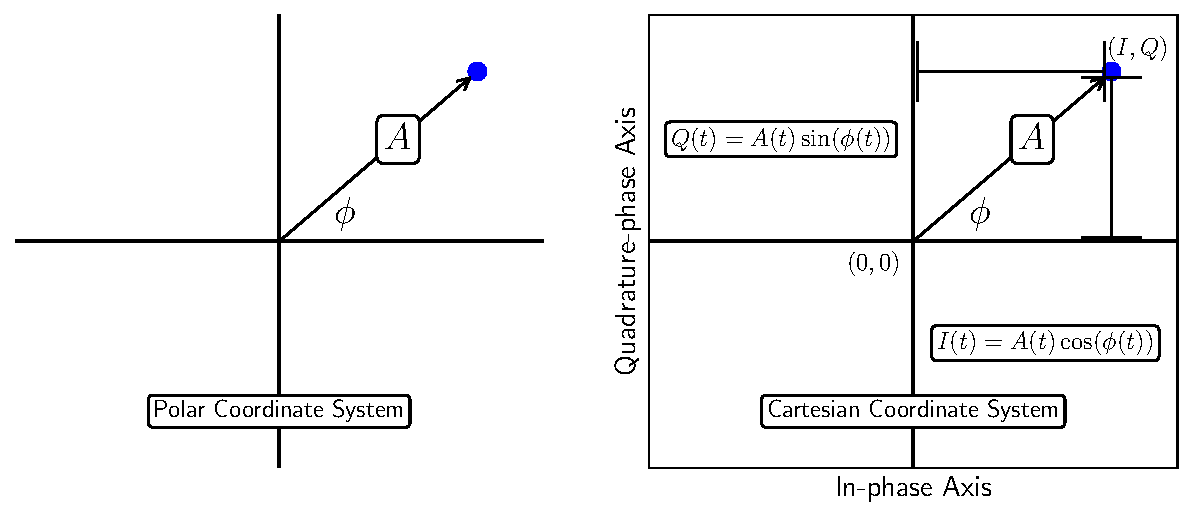
\includegraphics[width=280pt]{figures/iq-representation.pdf}
	\end{figure}

	\footnotesize

\end{frame}
%-------------------------------------------------------------------------------


%-------------------------------------------------------------------------------
\begin{frame}{SDR Hardware}  

\footnotesize
\textbf{RTL-SDR}

\begin{columns}

	\column{0.4\textwidth}

	\begin{figure}
		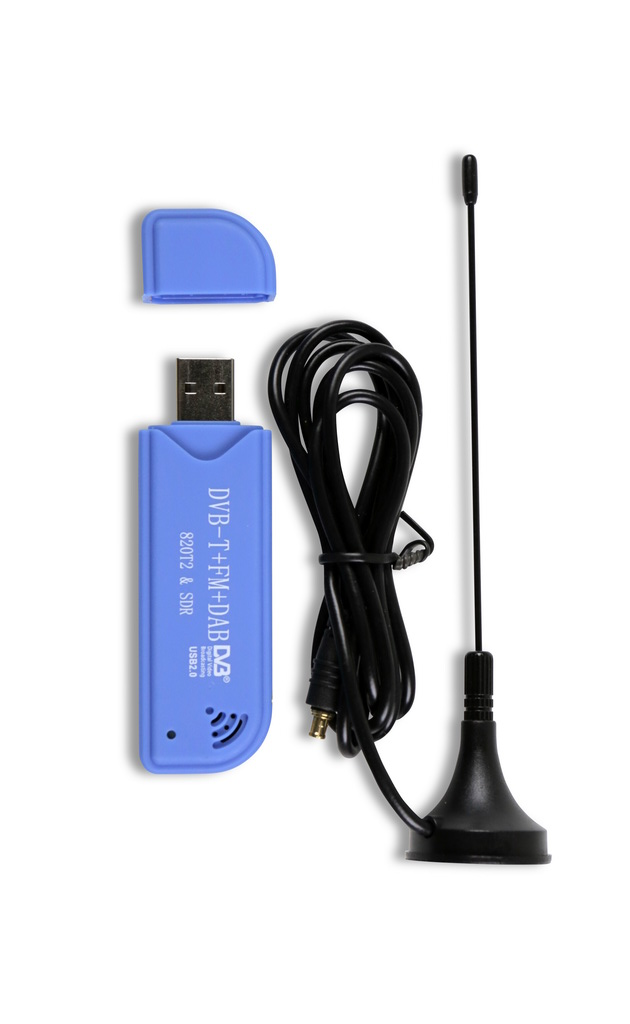
\includegraphics[width=100pt]{figures/rtl-sdr.jpg}
	\end{figure}

	\column{0.6\textwidth}

	\begin{itemize}
	\footnotesize
	\item A digital TV tuner repurposed as an SDR.
		\vspace{5pt}
	\item \emph{Realtek RTL2832U} and similar chips were discovered to be hackable.
		\vspace{5pt}
	\item The cheapest possible SDR you may find.
		\vspace{5pt}
	\item A wide variety of manufacturers; hence different variations of capabilities.
		\vspace{5pt}
	\item Sample rate is about 3.2 MHz
		\vspace{5pt}
	\item Tunable frequency range: 22 MHz -- 1 GHz.
		\vspace{5pt}
	\item Receive only; no transmission (simplex).
		\vspace{5pt}
	\item Read more: \url{https://www.rtl-sdr.com}
	\end{itemize}


\end{columns}

\end{frame}
%-------------------------------------------------------------------------------


%-------------------------------------------------------------------------------
\begin{frame}{SDR Hardware (cont.)}  

\footnotesize
\textbf{HackRF One}

\begin{columns}

	\column{0.4\textwidth}

	\begin{figure}
		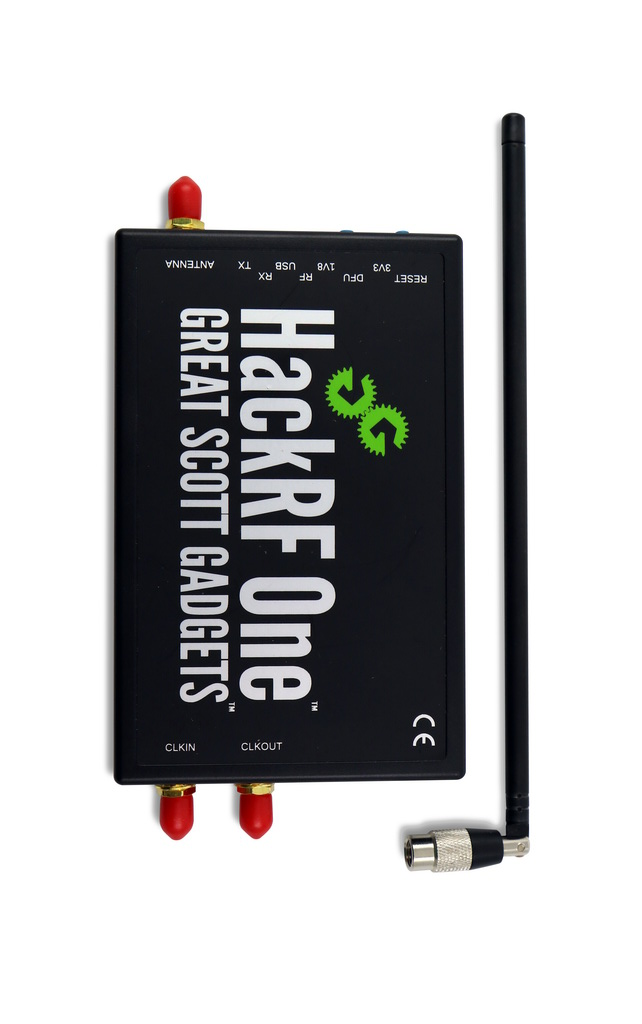
\includegraphics[width=120pt]{figures/hackrf-one.jpg}
	\end{figure}

	\column{0.6\textwidth}

	\begin{itemize}
	\footnotesize
	\item A purpose-built SDR device with a mid-range price tag.
		\vspace{5pt}
	\item Sample rate: upto 20 MHz.
		\vspace{5pt}
	\item Tunable frequency range: 1 MHz -- 6 GHz.
		\vspace{5pt}
	\item A wide range of antennas can be connect through the SMA connector.
		\vspace{5pt}
	\item Half-duplex: either transmit or receive at a given time.
		\vspace{5pt}
	\item Possible to time-synchronise with another device through clock input or output.
		\vspace{5pt}
	\item Read more: \url{https://greatscottgadgets.com/hackrf/one}
	\end{itemize}


\end{columns}

\end{frame}
%-------------------------------------------------------------------------------


%-------------------------------------------------------------------------------
\begin{frame}{SDR Software}  

\footnotesize
\textbf{GQRX}

	\begin{itemize}
	\footnotesize
	\item Easily view signals at different frequencies.
		\vspace{5pt}
	\item Facilitates live processing and saving observed signals.
		\vspace{5pt}
	\item Uses \emph{GNURadio} library underneath.
		\vspace{5pt}
	\item Launch it using \texttt{gqrx} command from the terminal.
	\end{itemize}

	\begin{figure}
		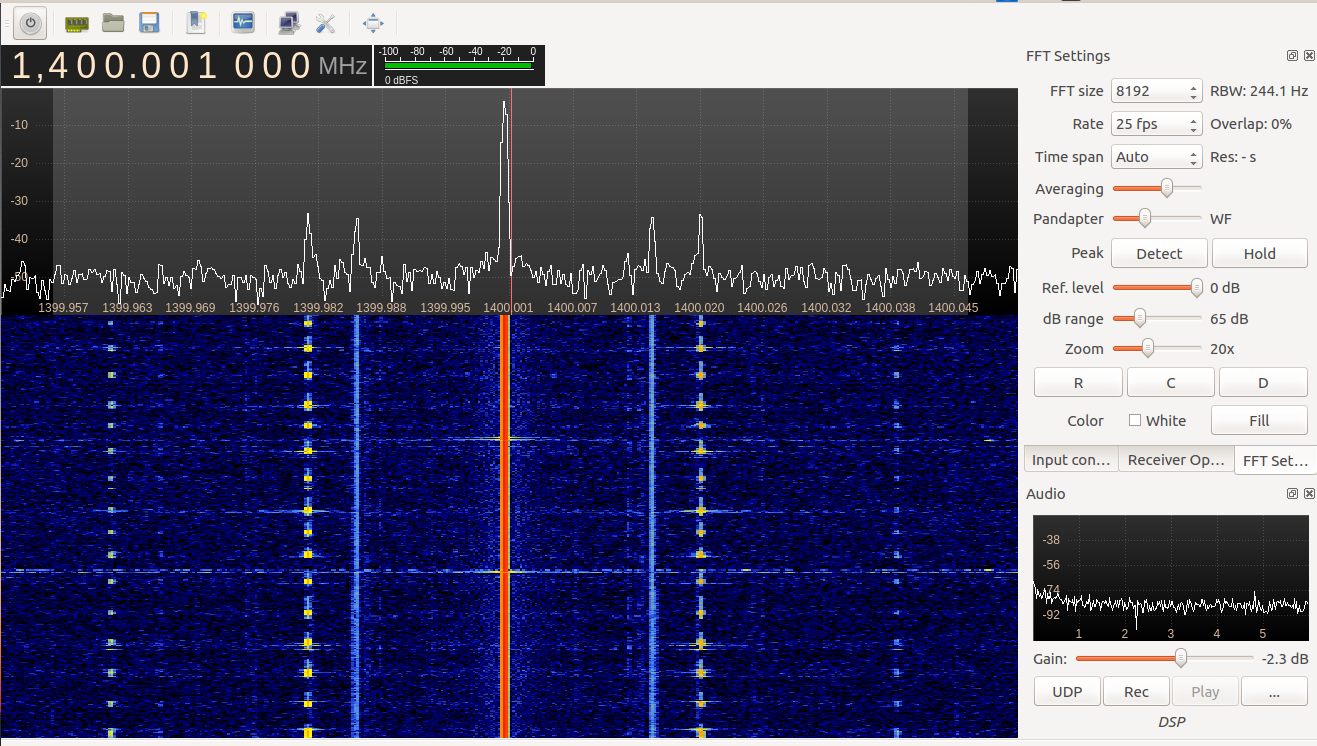
\includegraphics[width=200pt]{figures/gqrx-window.png}
	\end{figure}

\end{frame}
%-------------------------------------------------------------------------------


%-------------------------------------------------------------------------------
\begin{frame}{SDR Software (cont.)}  

\footnotesize
\textbf{GNURadio Companion (GRC)}

	\begin{itemize}
	\footnotesize
	\item Various signal processing blocks.
		\vspace{5pt}
	\item Custom build any application by creating flow graph using blocks.
		\vspace{5pt}
	\item Generates executable Python scripts for flow graphs, using \emph{GNURadio} library.
		\vspace{5pt}
	\item Launch it using \texttt{gnuradio-companion} command from the terminal.
	\end{itemize}

	\begin{figure}
		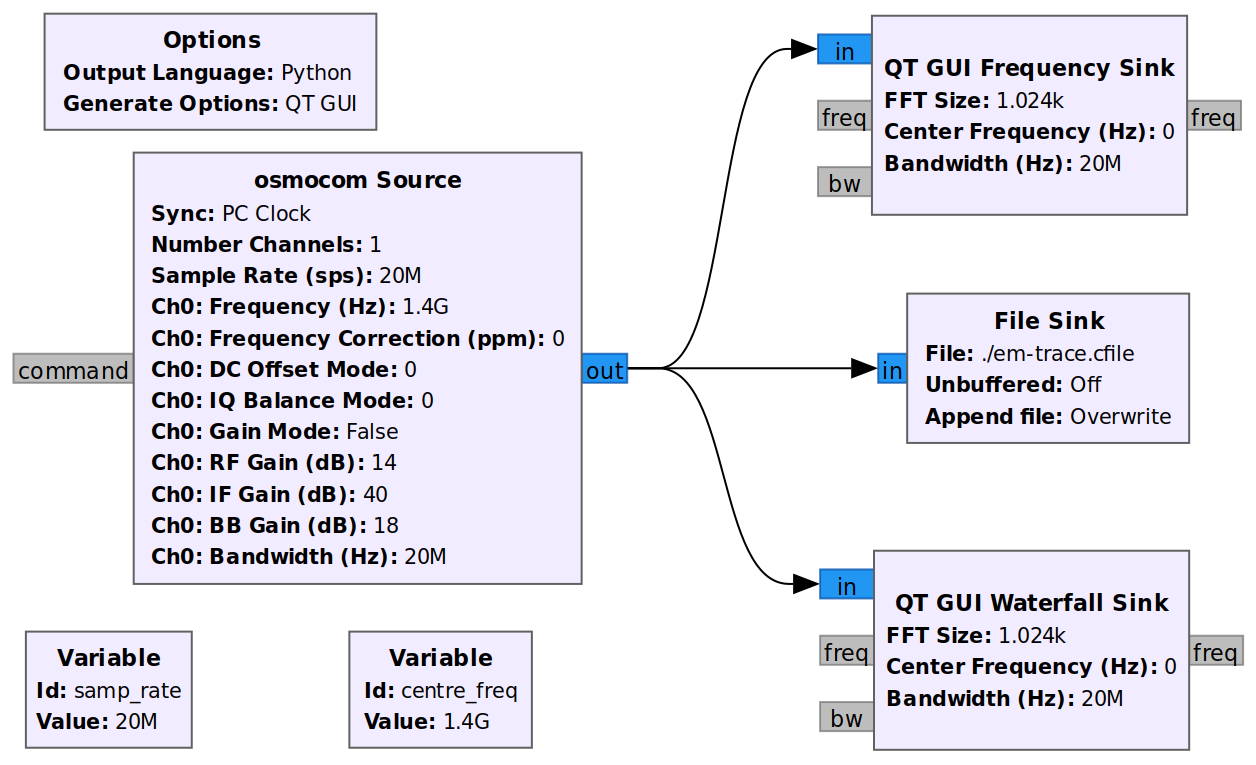
\includegraphics[width=200pt]{figures/grc-flowgraph-for-data-acquisition.png}
	\end{figure}

\end{frame}
%-------------------------------------------------------------------------------


%-------------------------------------------------------------------------------
\begin{frame}{Exercise 1}  

\footnotesize
Generating and visualising sine waves

	\begin{figure}
		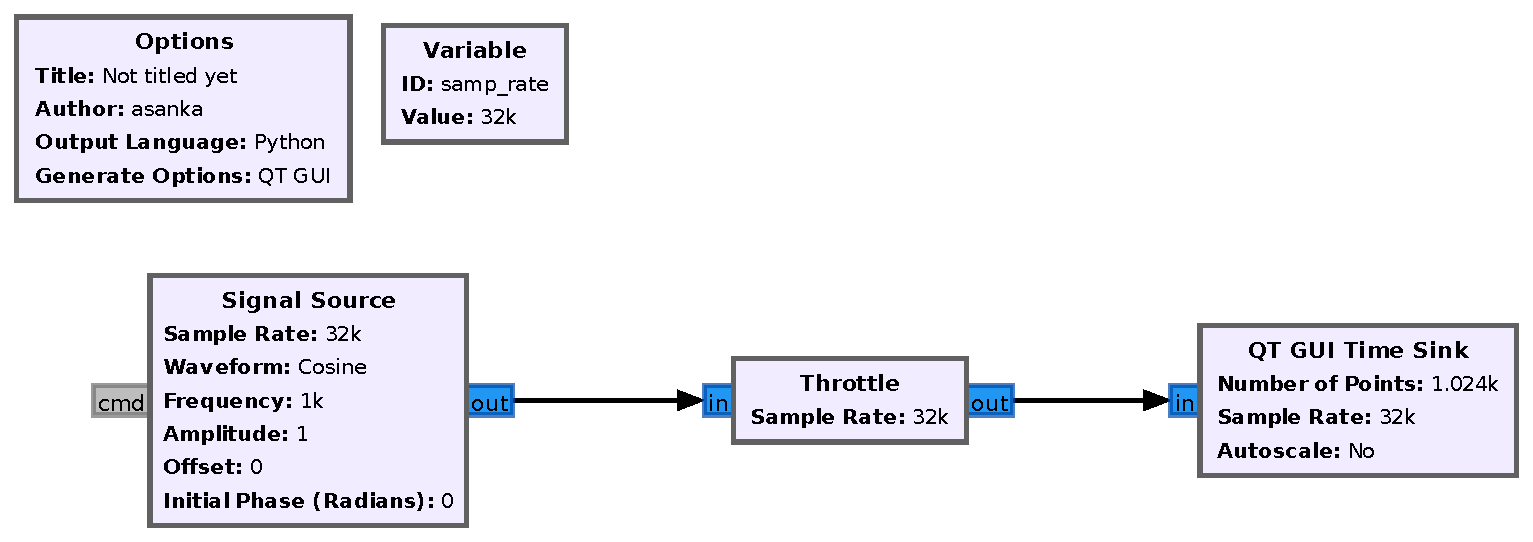
\includegraphics[width=300pt]{figures/Example-1.pdf}
	\end{figure}

\end{frame}
%-------------------------------------------------------------------------------


%-------------------------------------------------------------------------------
\begin{frame}{Exercise 2}  

\footnotesize
Generating and visualising noise

	\begin{figure}
		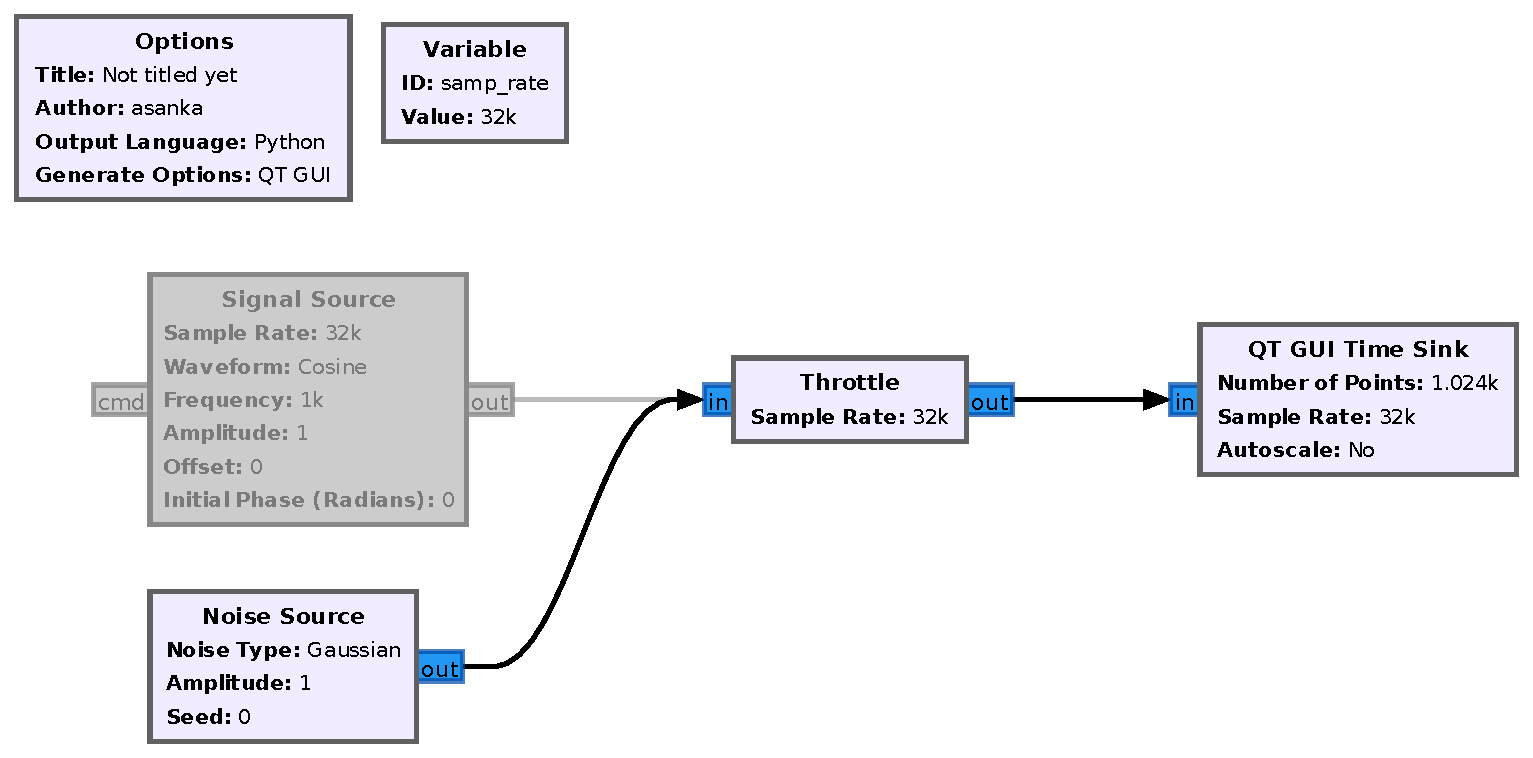
\includegraphics[width=300pt]{figures/Example-2.pdf}
	\end{figure}

\end{frame}
%-------------------------------------------------------------------------------


%-------------------------------------------------------------------------------
\begin{frame}{Exercise 3}  

\footnotesize
Capturing audio

	\begin{figure}
		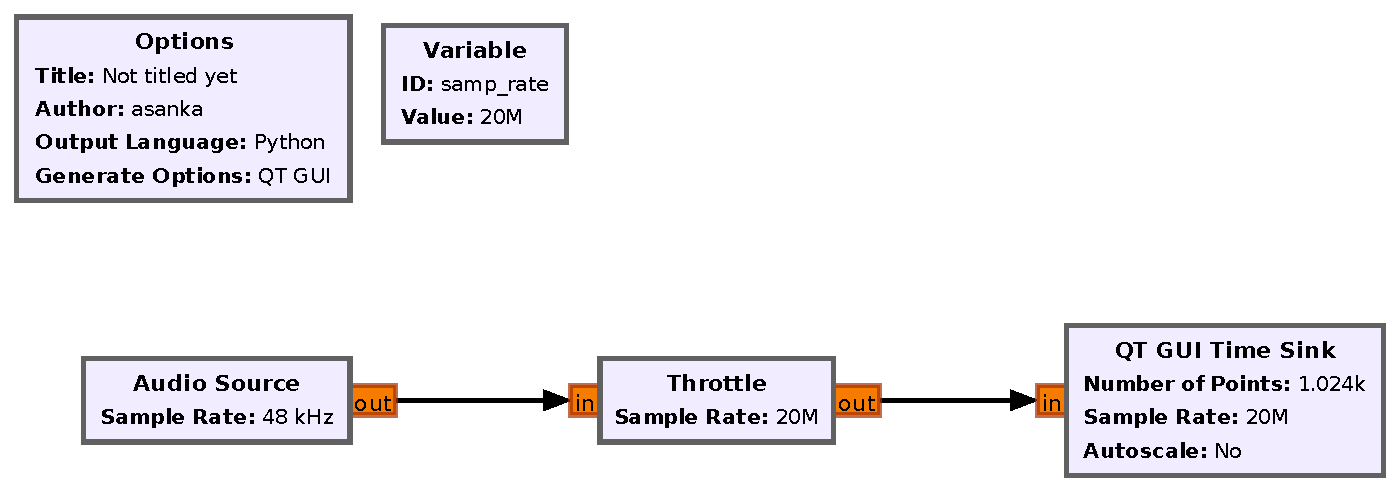
\includegraphics[width=300pt]{figures/Example-3.pdf}
	\end{figure}

\end{frame}
%-------------------------------------------------------------------------------


%-------------------------------------------------------------------------------
\begin{frame}{Exercise 4}  

\footnotesize
Visualising frequency domain

	\begin{figure}
		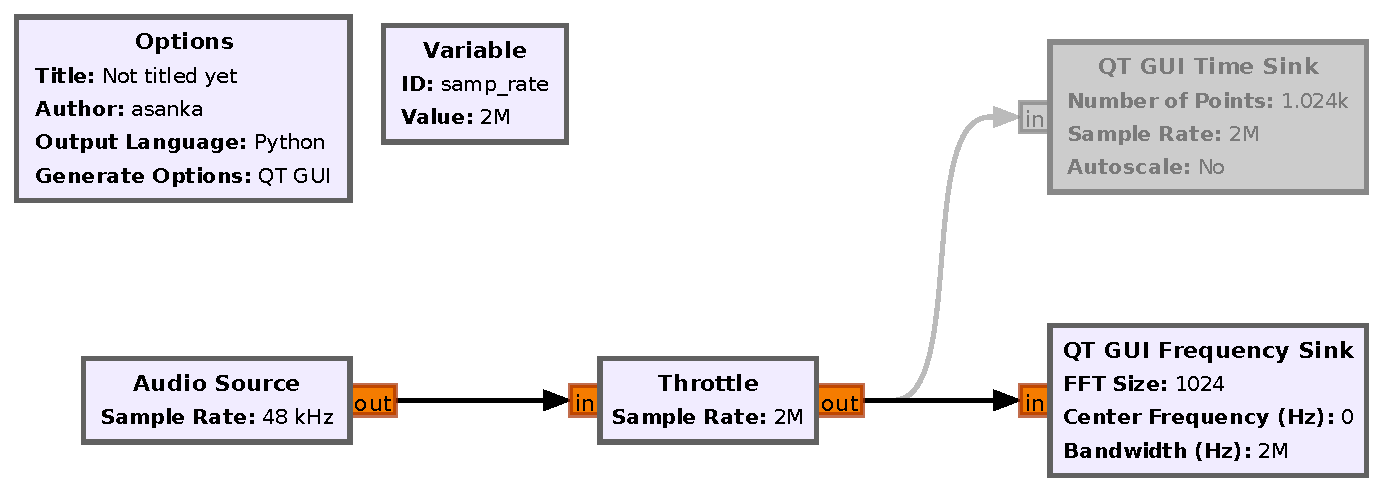
\includegraphics[width=300pt]{figures/Example-4.pdf}
	\end{figure}

\end{frame}
%-------------------------------------------------------------------------------


%-------------------------------------------------------------------------------
\begin{frame}{Exercise 5}  

\footnotesize
Spectrogarm/waterfall plot

	\begin{figure}
		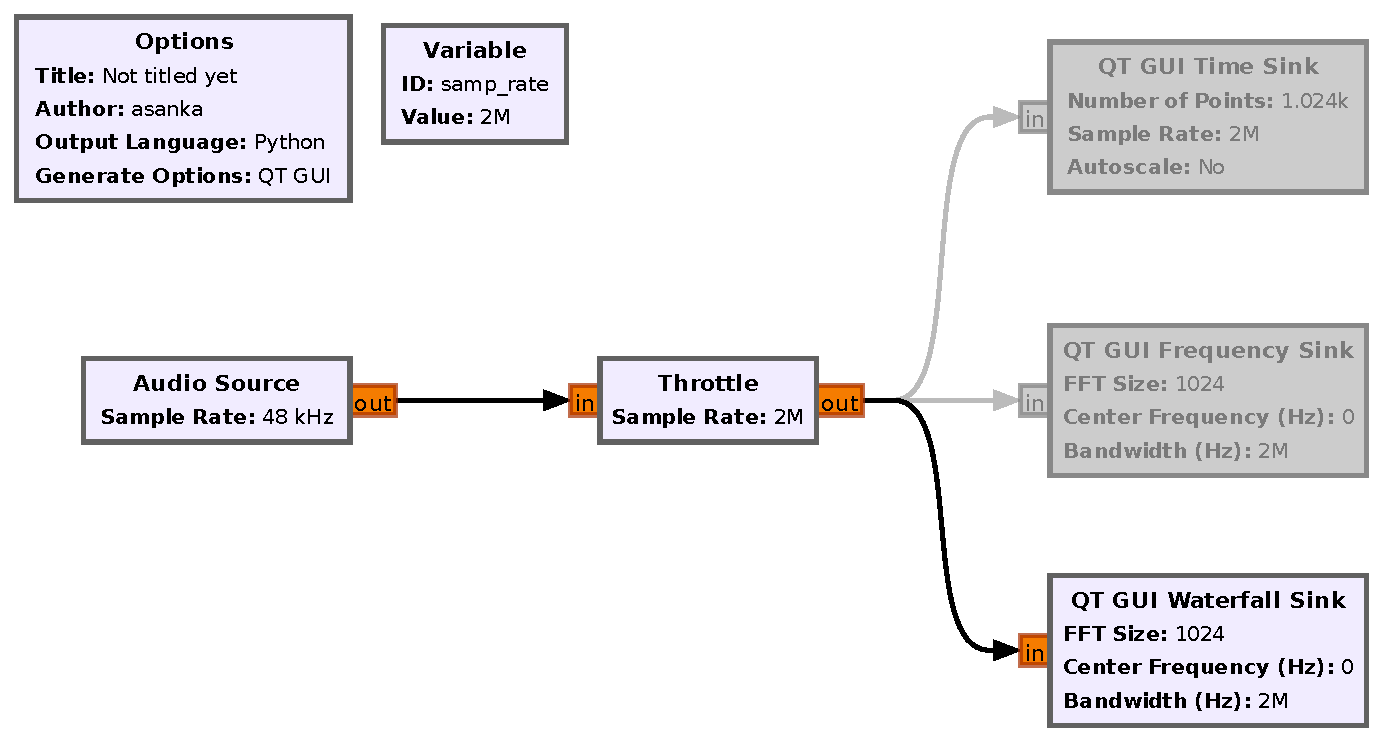
\includegraphics[width=300pt]{figures/Example-5.pdf}
	\end{figure}

\end{frame}
%-------------------------------------------------------------------------------


%-------------------------------------------------------------------------------
\begin{frame}{Exercise 6}  

\footnotesize
Saving data to (wav) files

	\begin{figure}
		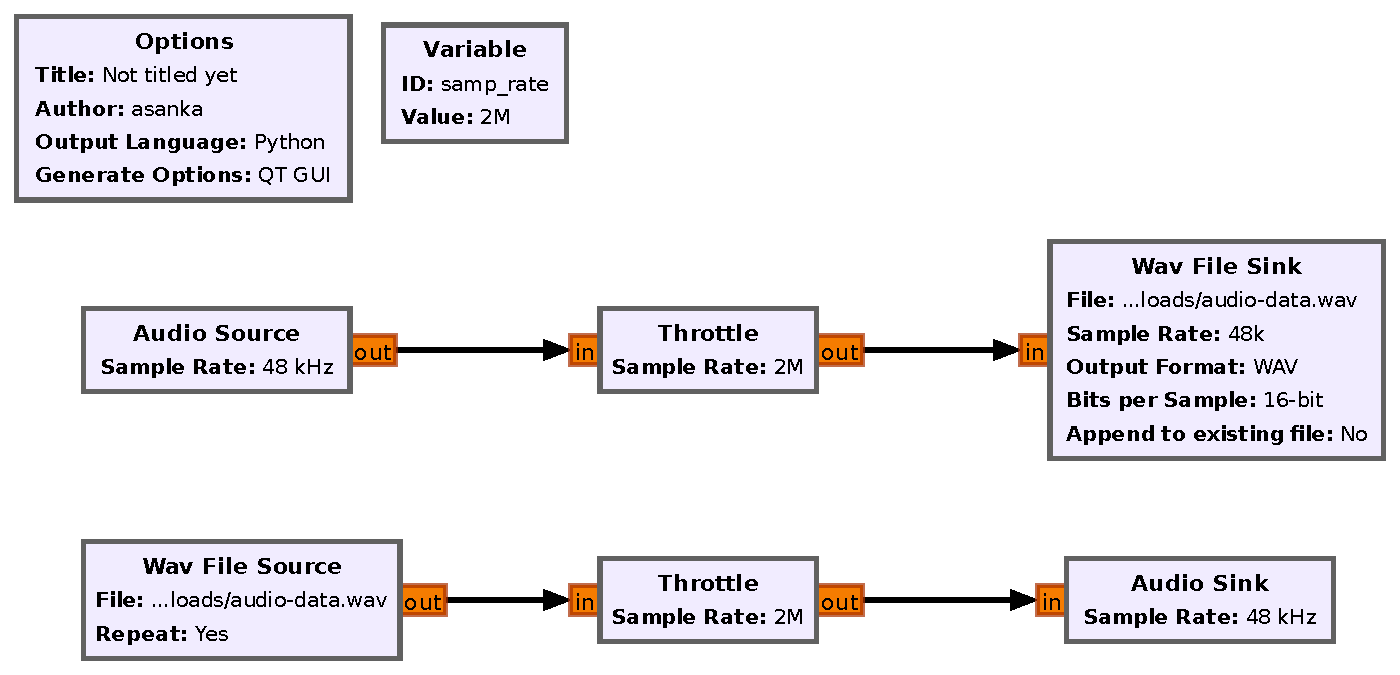
\includegraphics[width=300pt]{figures/Example-6.pdf}
	\end{figure}

\end{frame}
%-------------------------------------------------------------------------------


%-------------------------------------------------------------------------------
\begin{frame}{Exercise 7}  

\footnotesize
TCP connections between flowgraphs

	\begin{figure}
		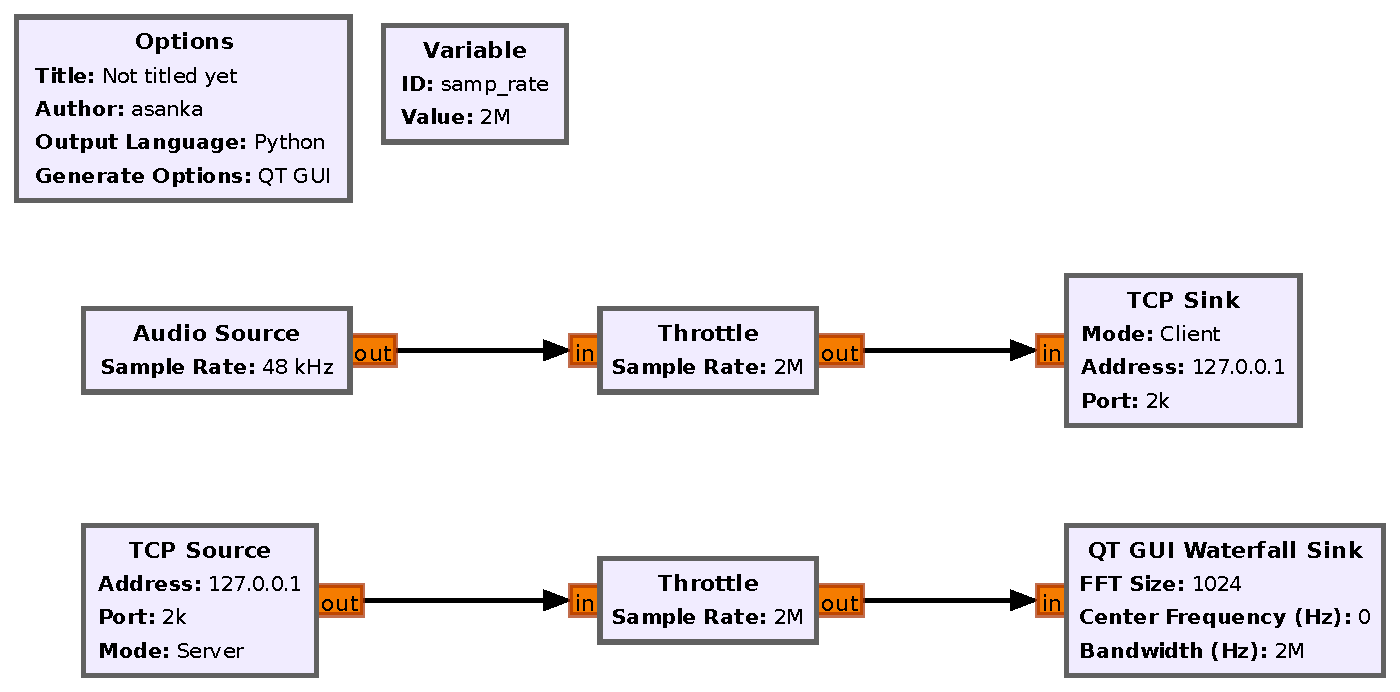
\includegraphics[width=300pt]{figures/Example-7.pdf}
	\end{figure}

\end{frame}
%-------------------------------------------------------------------------------


%-------------------------------------------------------------------------------
\begin{frame}{Exercise 8}  

\footnotesize
Capturing data from HackRF

	\begin{figure}
		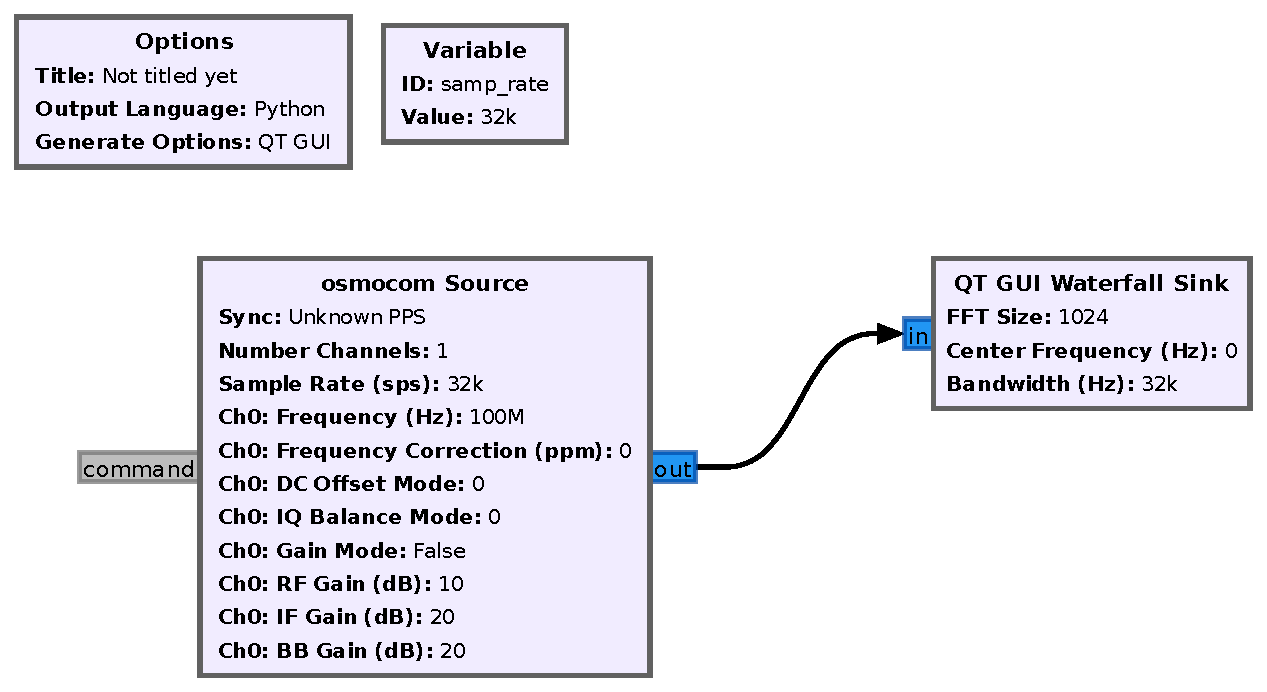
\includegraphics[width=300pt]{figures/Example-8.pdf}
	\end{figure}

\end{frame}
%-------------------------------------------------------------------------------


%-------------------------------------------------------------------------------
\begin{frame}{Exercise 9}  

\footnotesize
Additional GUI components

	\begin{figure}
		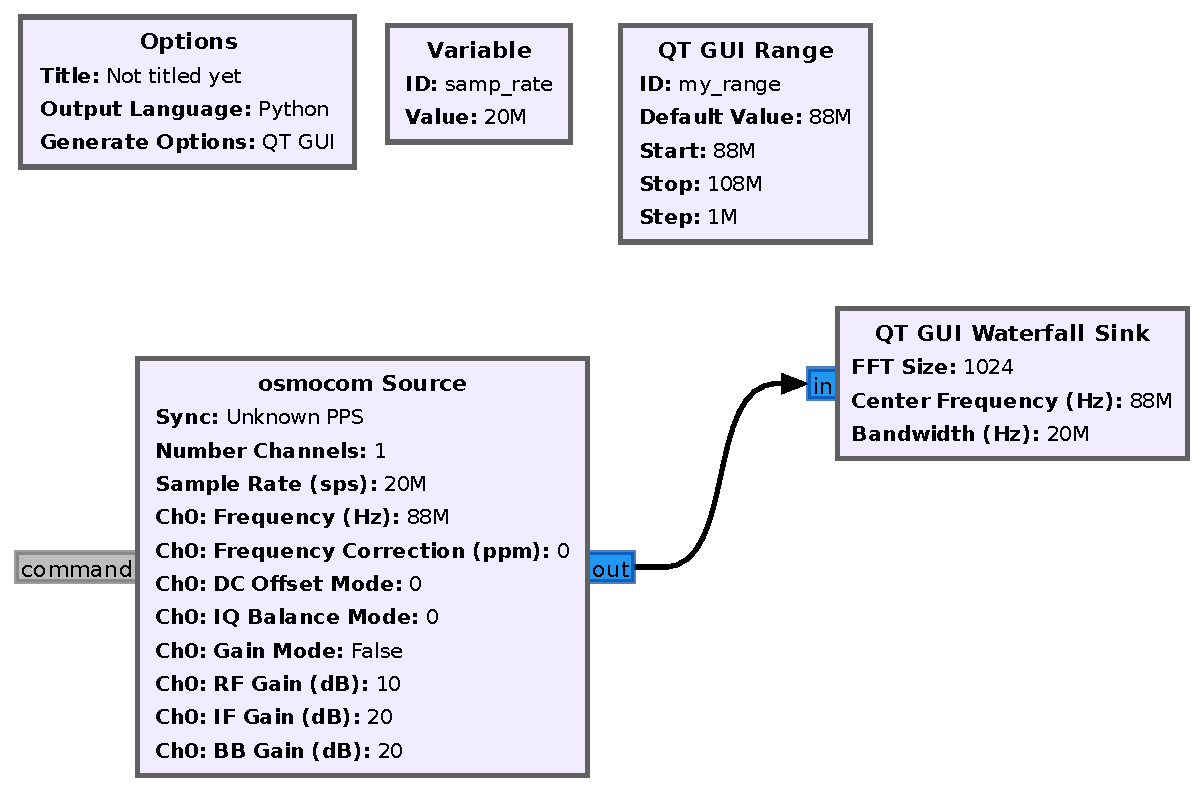
\includegraphics[width=300pt]{figures/Example-9.pdf}
	\end{figure}

\end{frame}
%-------------------------------------------------------------------------------


%-------------------------------------------------------------------------------
\begin{frame}{Exercise 10}  

\footnotesize
Let's link the HackRF connected to my computer with a GRC flow graph on your computer through TCP.

\vspace{10pt}

	This setup will be useful for us to complete the exercises in the next segment of the workshop, i.e., Part 4.

\end{frame}
%-------------------------------------------------------------------------------



%-------------------------------------------------------------------------------
\begin{frame}{}  

	\begin{block}{Part 3}
	\end{block}

\end{frame}
%-------------------------------------------------------------------------------


%-------------------------------------------------------------------------------
\begin{frame}{Capturing EM Side-Channel Radiation}  

	\begin{itemize}
	\footnotesize
	\item Our key focus is EM radiation from the processor/microcontroller/SoC.
		\vspace{5pt}
	\item Strongest signals are in the clock frequency or its harmonics.
		\vspace{5pt}
	\item Signal acquisition should be performed as closer to the target chip as possible.
		\vspace{5pt}
	\item Magnetic H-loop antennas are more suitable for the job.
	\end{itemize}


	\begin{figure}
		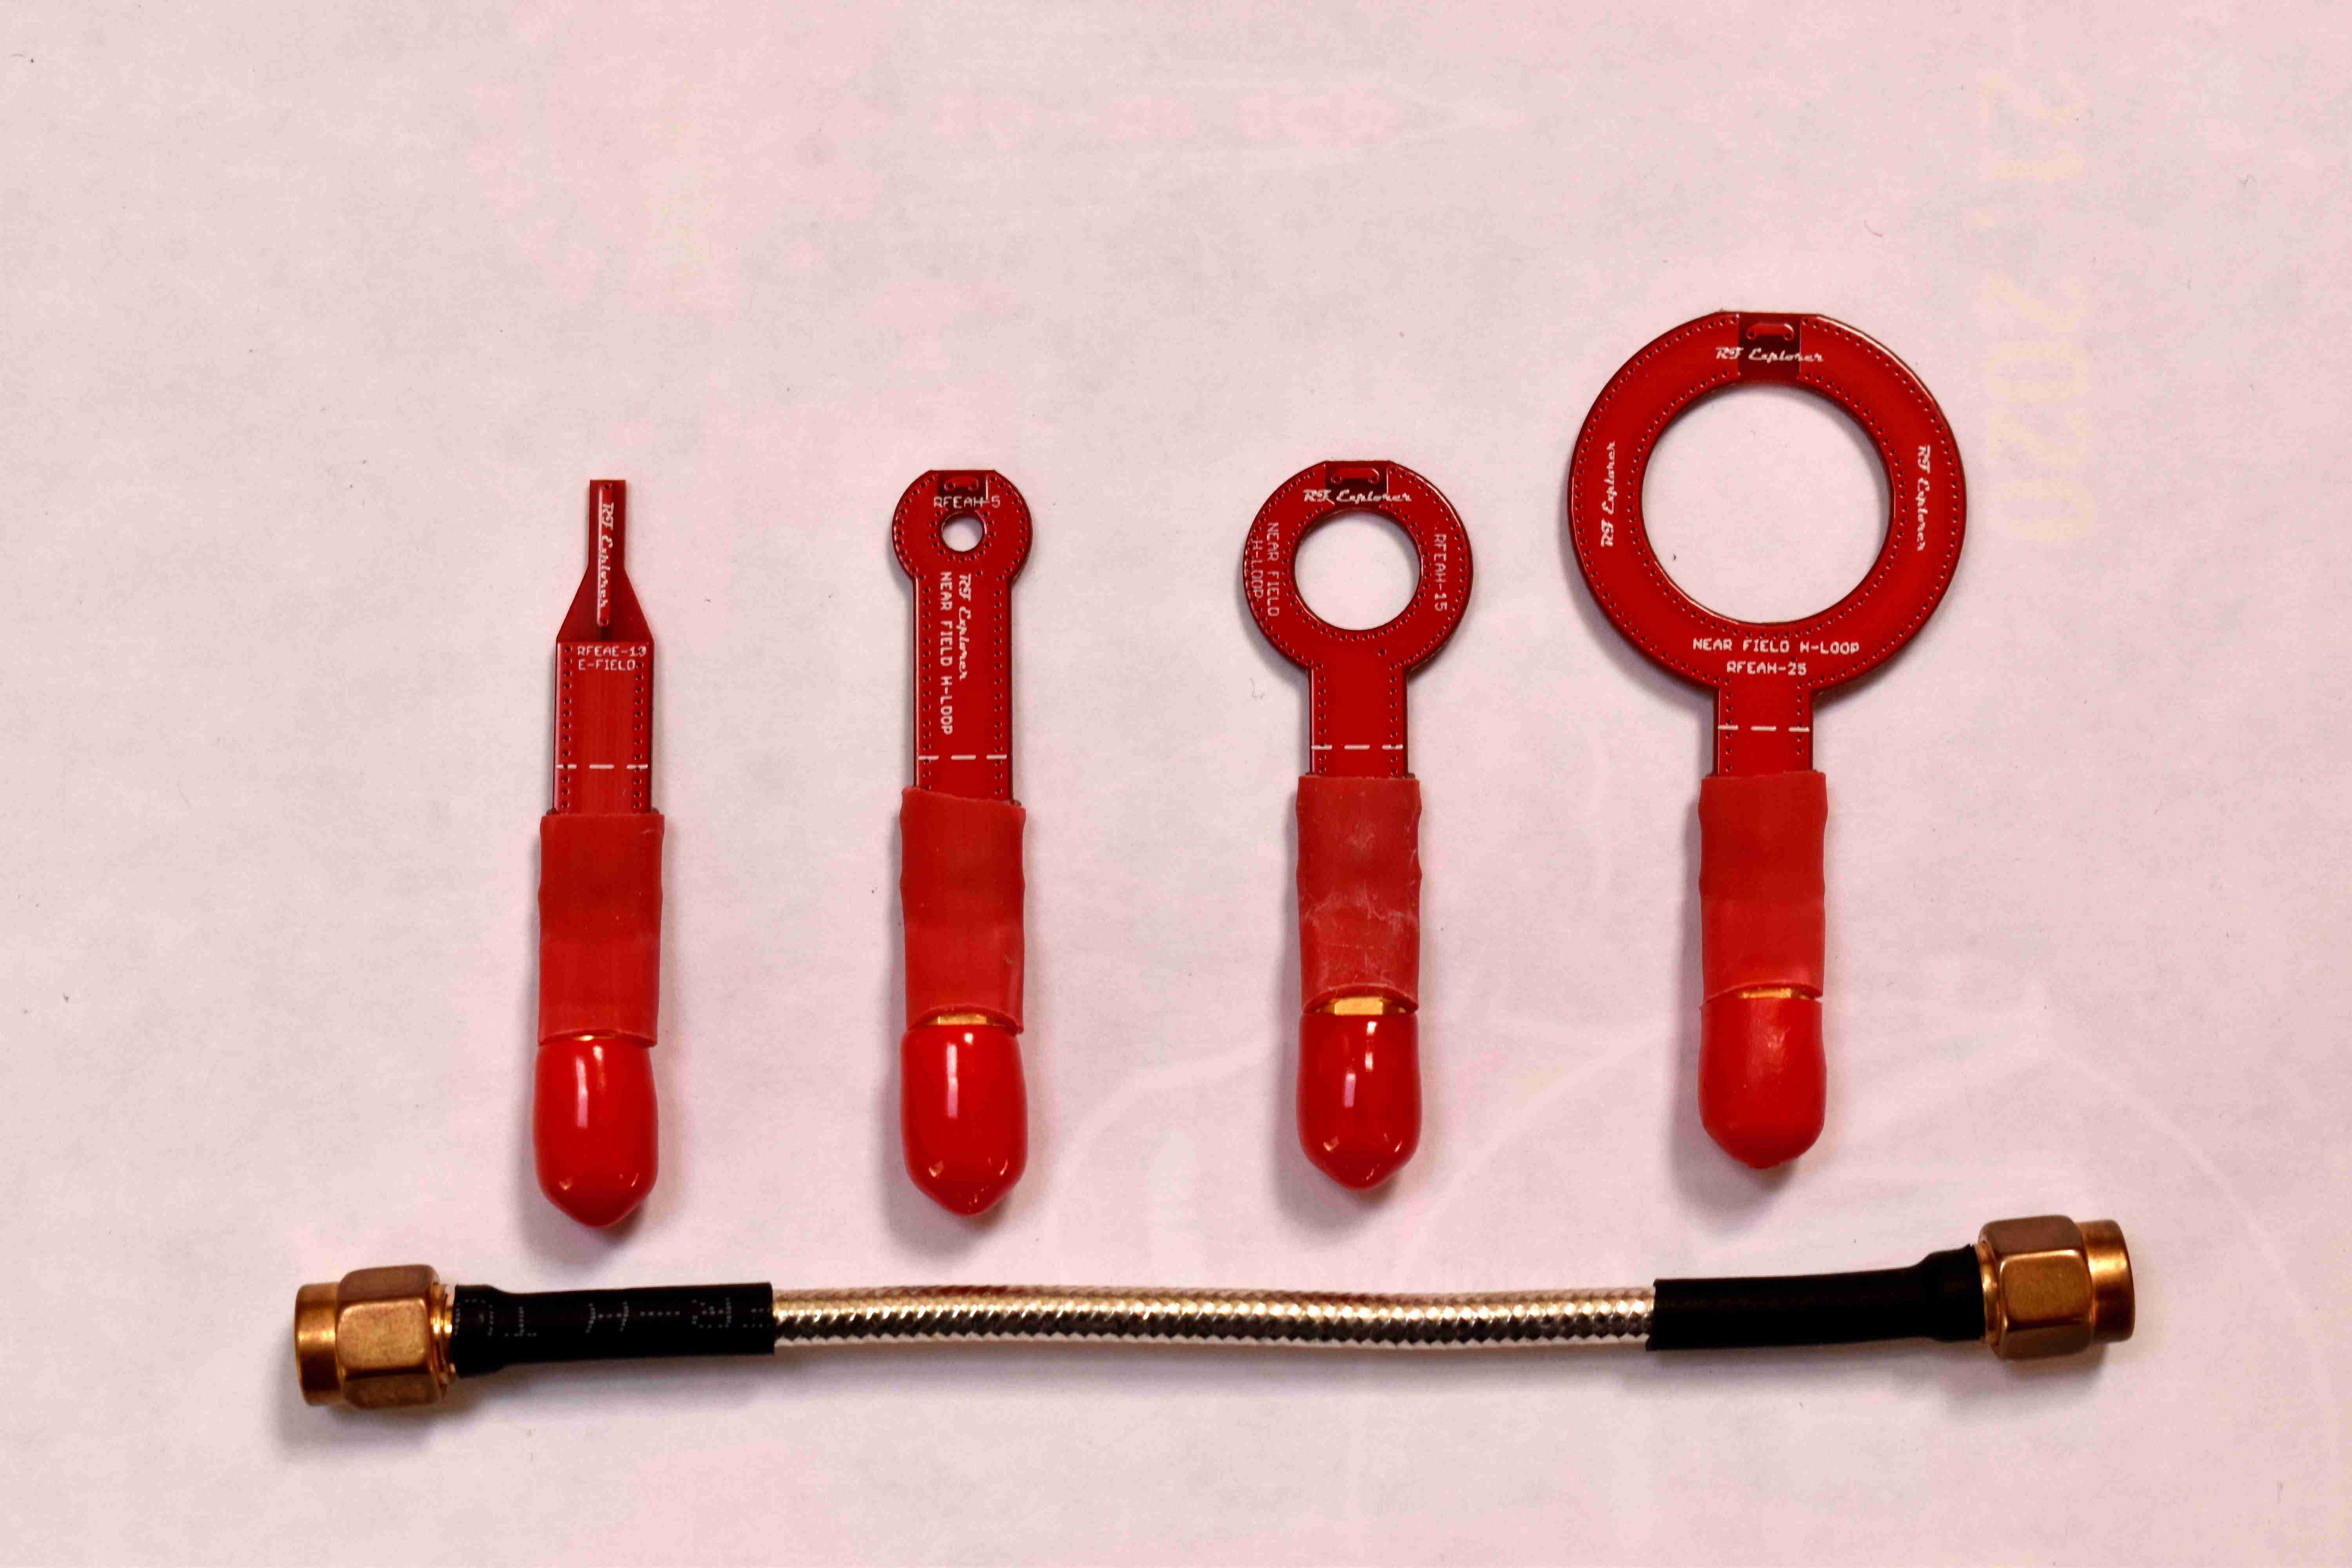
\includegraphics[width=140pt]{figures/antenna-kit-small.jpg}
	\end{figure}

\end{frame}
%-------------------------------------------------------------------------------



%-------------------------------------------------------------------------------
\begin{frame}{Capturing EM Side-Channel Radiation (cont.)}  

\footnotesize
\textbf{Passive acquisition:}

	\begin{figure}
		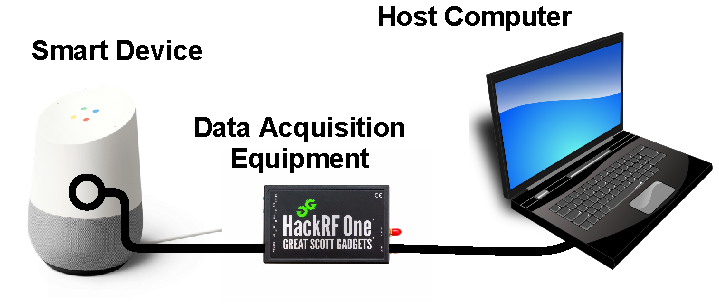
\includegraphics[width=210pt]{figures/hardware-setup.pdf}
	\end{figure}

\end{frame}
%-------------------------------------------------------------------------------


%-------------------------------------------------------------------------------
\begin{frame}{Capturing EM Side-Channel Radiation (cont.)}  

\footnotesize
\textbf{Instrumented acquisition:}

	\begin{figure}
		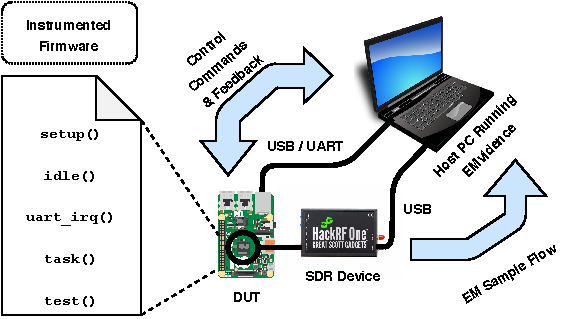
\includegraphics[width=210pt]{figures/signal-acquisition-2.pdf}
	\end{figure}

\end{frame}
%-------------------------------------------------------------------------------


%-------------------------------------------------------------------------------
\begin{frame}{Capturing EM Side-Channel Radiation (cont.)}  

\footnotesize
\textbf{Arduino and Raspberry Pi}

	\begin{figure}
		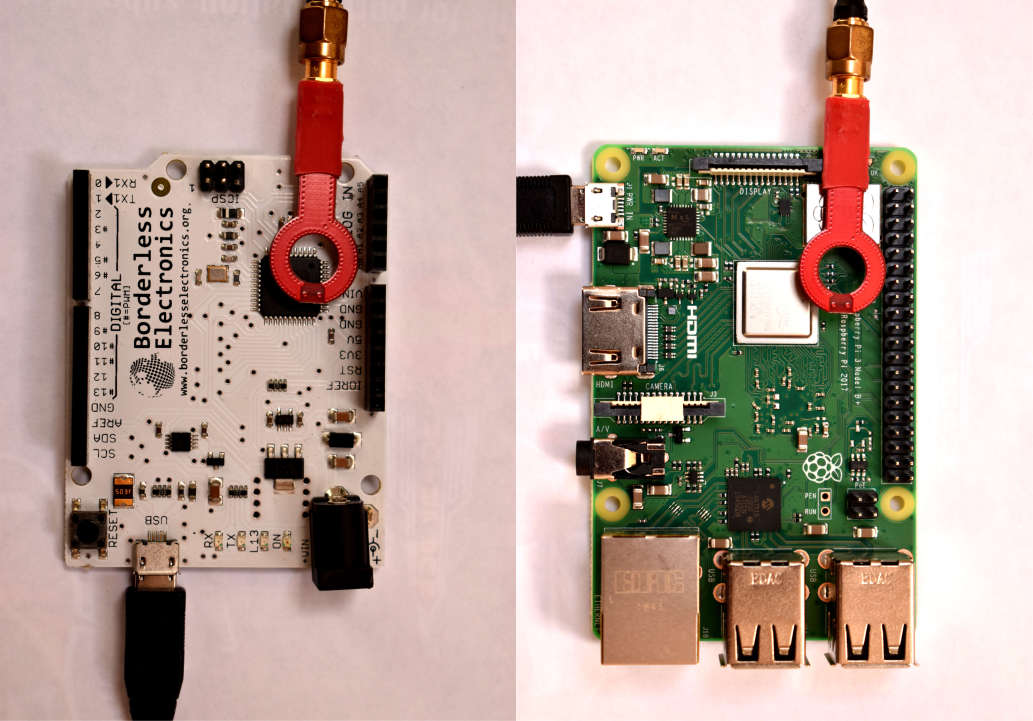
\includegraphics[width=200pt]{figures/arduino-rpi-with-antenna.jpg}
	\end{figure}

\end{frame}
%-------------------------------------------------------------------------------


%-------------------------------------------------------------------------------
\begin{frame}{Capturing EM Side-Channel Radiation (cont.)}  

\footnotesize
\textbf{Smartphone}

	\begin{figure}
		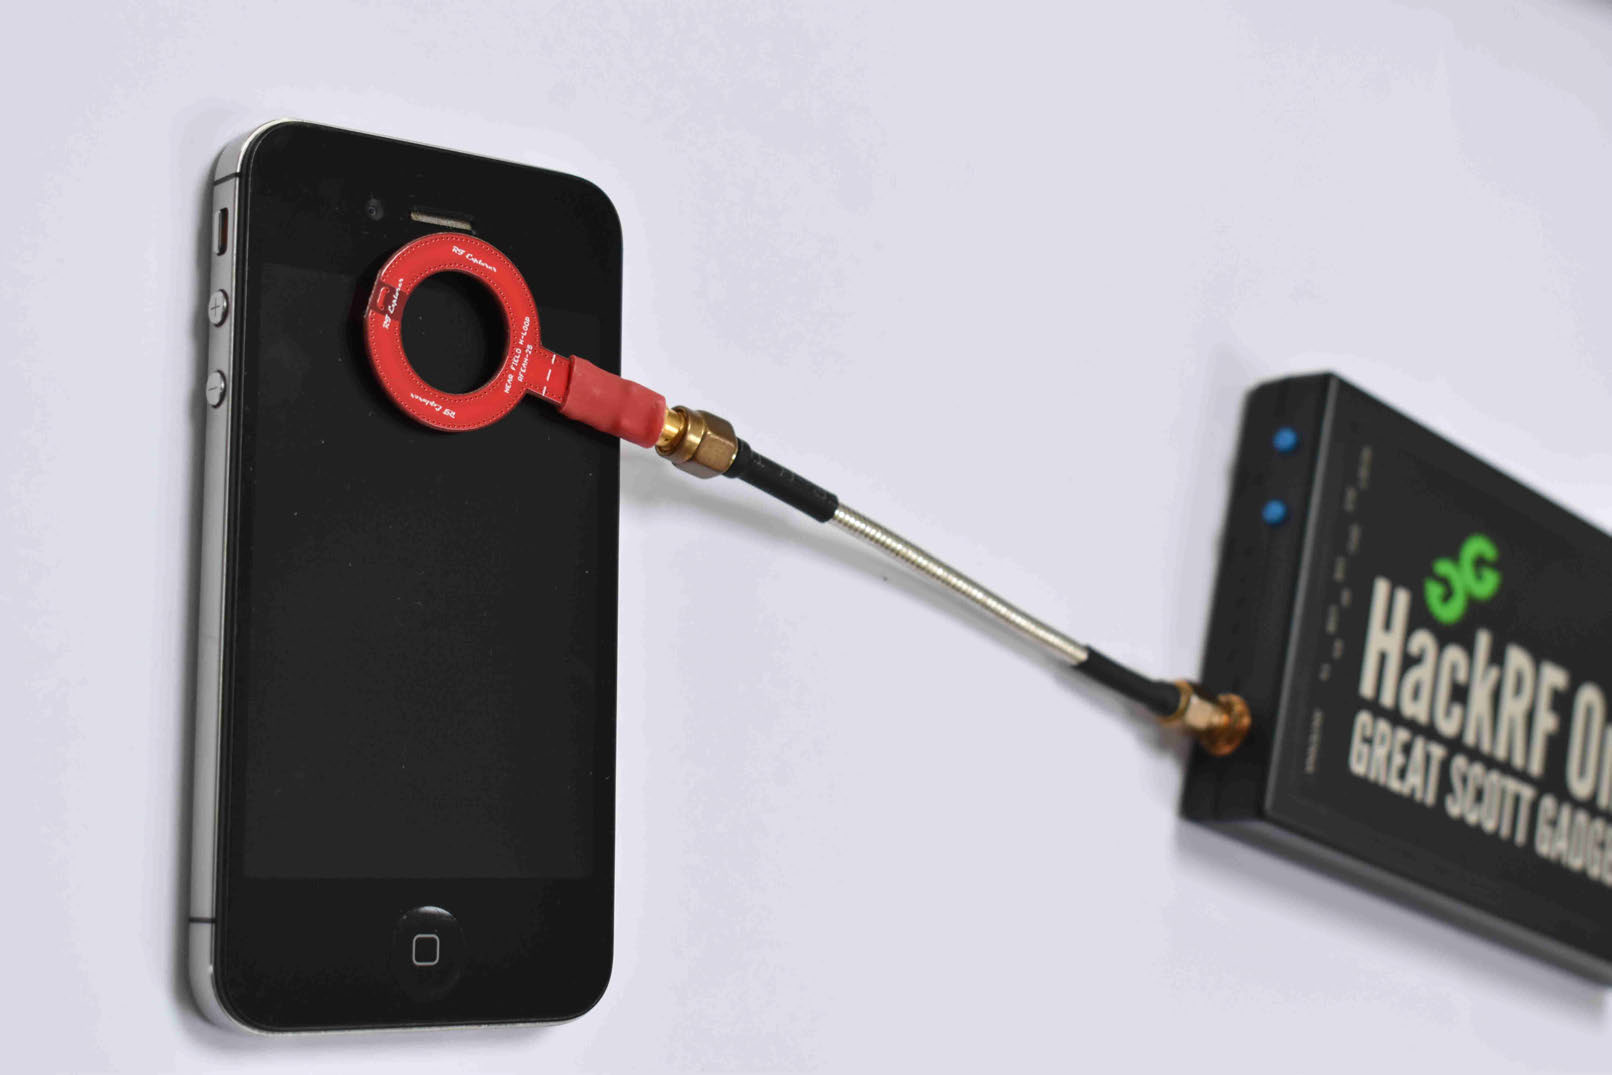
\includegraphics[width=200pt]{figures/iphone-hackrf.png}
	\end{figure}

\end{frame}
%-------------------------------------------------------------------------------


%-------------------------------------------------------------------------------
\begin{frame}{Processing EM Side-Channel Data}  

\begin{itemize}
\footnotesize
	\item Once the EM radiation from a target device --- device-under-test (DUT) --- is captured, we can process it.
		\vspace{10pt}
	\item GNURadio Companion flowgraphs have blocks for signal processing, but it is not sufficient.
		\vspace{10pt}
	\item The ideal way is to process data using a scientific computing language, such as Python.
		\vspace{10pt}
	\item Once the EM data is loaded into a \emph{numpy} array, the possibilities are endless.
\end{itemize}

\end{frame}
%-------------------------------------------------------------------------------


%-------------------------------------------------------------------------------
\begin{frame}[fragile]{Processing EM Side-Channel Data (cont.)}

\footnotesize
\textbf{Loading I/Q data into Python:}
\vspace{30pt}

\begin{minted}{python}
import numpy as np
import matplotlib.pyplot as plt

def getData(cfileName):
    data = np.fromfile(cfileName, dtype="float32")
    data = data[0::2] + 1j*data[1::2]
    return data

data = getData("/home/asanka/Desktop/my-data.cfile")
\end{minted}

\end{frame}
%-------------------------------------------------------------------------------


%-------------------------------------------------------------------------------
\begin{frame}[fragile]{Processing EM Side-Channel Data (cont.)}

\footnotesize
\textbf{Plotting I/Q data in Python:}
\vspace{30pt}

\begin{minted}{python}
fig = plt.figure()
plt.psd(data, NFFT=2048, Fs=20e6)
plt.show()


fig = plt.figure()
pxx, freq, t, cax = plt.specgram(data, NFFT=1024, Fs=20e6, 
	Fc=88e6, mode='magnitude')
fig.colorbar(cax).set_label('Intensity [dB]')
plt.xlabel("Time (s)")
plt.ylabel("Frequency (Hz)")
plt.show()
\end{minted}

\end{frame}
%-------------------------------------------------------------------------------


%-------------------------------------------------------------------------------
\begin{frame}{Activity}  

\begin{itemize}
\footnotesize
	\item Let's use EM side-channel emission of a DUT to determine whether the device is powered up or not.
		\vspace{10pt}
	\item Our model DUT is an Arduino Uno.
		\vspace{10pt}
	\item You can write a program to the Arduino Uno to perform some task.
		\vspace{10pt}
	\item Collect EM trace data for the two cases: the Arduino is powered off and running your program.
		\vspace{10pt}
	\item Visualise the two EM traces. Can you observe a difference?
		\vspace{10pt}
	\item Explore whether you can automate the detection process programmatically. You can use various approaches, such as digital signal processing, statists, machine learning, etc.
\end{itemize}

\end{frame}
%-------------------------------------------------------------------------------



%-------------------------------------------------------------------------------
\begin{frame}{}  

	\begin{block}{Part 4}
	\end{block}

\end{frame}
%-------------------------------------------------------------------------------

%-------------------------------------------------------------------------------
\begin{frame}{Analysing EM Dataset}  

\footnotesize
The pipeline from capturing EM data to analysis...

	\begin{figure}
		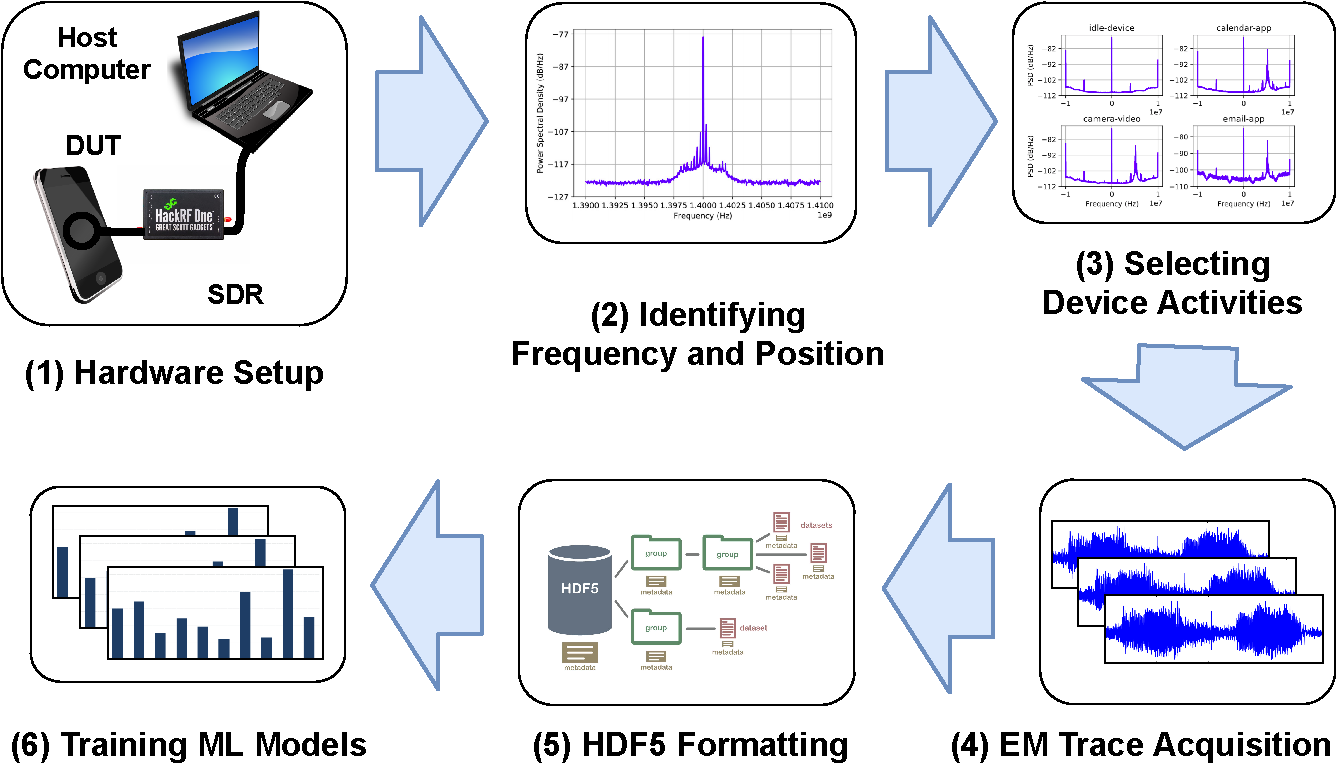
\includegraphics[width=230pt]{figures/sdr-data-pipeline-V2.pdf}
	\end{figure}

\end{frame}
%----------------------------------------------------------------------


%-------------------------------------------------------------------------------
\begin{frame}{Analysing EM Dataset}  

\footnotesize
\textbf{Huge Size of the Data Files}
		\vspace{10pt}

	\begin{itemize}
	\item In GNU Radio library, two 32 bit (4 byte) floating point values are used to represent a complex I/Q sample.
		\vspace{10pt}
	\item Therefore, each EM data sample is a 8 bytes long complex value.
		\vspace{10pt}
	\item Consider if we sampled data at the maximum sample rate of HackRF One device (i.e., 20 MHz) using GNURadio library to save data.
		\vspace{10pt}
	\item Size of data per second = $8$ bytes $\times 20 \times 10^{6} = 160$ MB
		\vspace{10pt}
	\item Size of data for 10 seconds = $160$ MB $\times 10 = 1.6$ GB
	\end{itemize}

\end{frame}
%----------------------------------------------------------------------


%-------------------------------------------------------------------------------
\begin{frame}{Analysing EM Dataset (cont.)}  

\footnotesize
The specifications of devices in the dataset:
	

	\begin{figure}
		\includegraphics[width=250pt]{figures/device-spec-from-the-dataset.png}
	\end{figure}

\end{frame}
%--------------------------------------


%-------------------------------------------------------------------------------
\begin{frame}{Analysing EM Dataset (cont.)}  

	\footnotesize
	Structure of the dataset in HDF5 file format (em-dataset.h5):

	\begin{figure}
		\includegraphics[width=280pt]{figures/hdf5-dataset-structure.pdf}
	\end{figure}

\end{frame}
%--------------------------------------

%-------------------------------------------------------------------------------
\begin{frame}{Analysing EM Dataset (cont.)}  

	\footnotesize
	Amazon Echo Dot -- Power Spectral Density (PSD) Plots

	\begin{figure}
		\includegraphics[width=240pt]{figures/amazon-echo-dot-psd-plots.pdf}
	\end{figure}

\end{frame}
%--------------------------------------


%-------------------------------------------------------------------------------
\begin{frame}{Analysing EM Dataset (cont.)}  

	\footnotesize
	Nokia 4.2 -- Histogram

	\begin{figure}
		\includegraphics[width=240pt]{figures/data-distribution-plots-Nokia42.pdf}
	\end{figure}

\end{frame}
%--------------------------------------


%-------------------------------------------------------------------------------
\begin{frame}{Analysing EM Dataset (cont.)}  

	\begin{itemize}
	\footnotesize
	\item Go ahead and launch Jupyter Notebook inside the downloaded Git repository.
		\vspace{10pt}
	\item We'll explore the code examples for the following things:
		\vspace{10pt}
		\begin{enumerate}
		\footnotesize
		\item Reading and basic visualisation of EM data.
		\vspace{5pt}
		\item Preprocessing EM data for feature extraction.
		\vspace{5pt}
		\item Simple machine learning classifiers to distinguish software behaviour.
		\end{enumerate}
	\end{itemize}

\end{frame}
%-------------------------------------------------------------------------------


%-------------------------------------------------------------------------------
%\begin{frame}{Build Your Arduino Classifier}

%\begin{itemize}
%\footnotesize
%\item Shall we collect our own data and build a classifier for software behaviour detection?
%\vspace{10pt}
%\item We can program an Arduino Uno to do two different tasks and capture two EM data files representing each task.
%\vspace{10pt}
%\item Let's see if we can build a simple classifier to distinguish between the two tasks.
%\end{itemize}

%\end{frame}
%-------------------------------------------------------------------------------


%-------------------------------------------------------------------------------
\begin{frame}{Conclusion}

\begin{itemize}
\footnotesize
\item EM-SCA for digital forensic insight acquisition is still in its early days.
\vspace{10pt}
\item Loads of technical and scientific problems remaining to be solves; great for research!
\vspace{10pt}
\item \emph{Cross-device portability} of trained models.
\vspace{10pt}
\item No need to possess hardware equipment to conduct research in this area; datasets are available to work on (from our group and many others).
\vspace{10pt}
\item Thank you for your participation. Feel free to get in touch: \\ 
	\vspace{5pt} 
	Asanka Sayakkara (\texttt{asa@ucsc.cmb.ac.lk})
\end{itemize}

\end{frame}
%-------------------------------------------------------------------------------


%-------------------------------------------------------------------------------
\begin{frame}{References}

\begin{enumerate}
\scriptsize
\item Asanka Sayakkara, Le-Khac, N-A., and Scanlon, M., ``Electromagnetic Side-Channel Attacks: Potential for Progressing Hindered Digital Forensic Analysis", International Workshop on Speculative Side Channel Analysis (WoSSCA 2018), Amsterdam, Netherlands, July 2018.
\vspace{10pt}
\item Asanka Sayakkara, Le-Khac, N-A., and Scanlon, M., ``A Survey of Electromagnetic Side-Channel Attacks and Discussion on their Case-Progressing Potential for Digital Forensics", Elsevier Digital Investigation, 2019. 
\vspace{10pt}
\item Asanka Sayakkara, Le-Khac, N-A., and Scanlon, M., ``Leveraging Electromagnetic Side-Channel Analysis for the Investigation of IoT Devices", DFRWS USA, Portland, OR, USA, July 2019.
\vspace{10pt}
\item Asanka Sayakkara and Nhien-An Le-Khac , ``Electromagnetic Side-Channel Analysis for IoT Forensics: Challenges, Framework, and Datasets," in IEEE Access, vol 9, pp. 113585-113598, 2021. 
\vspace{10pt}
\item[] Find more here: \url{https://www.asayakkara.org/publications.html}
\end{enumerate}

\end{frame}
%-------------------------------------------------------------------------------



\end{document}


